% Options for packages loaded elsewhere
\PassOptionsToPackage{unicode}{hyperref}
\PassOptionsToPackage{hyphens}{url}
\PassOptionsToPackage{dvipsnames,svgnames*,x11names*}{xcolor}
%
\documentclass[
  11pt,
]{article}

%Additions
\newif\iftimestamp
\timestampfalse
%

\usepackage{lmodern}
\usepackage{amssymb,amsmath}
\usepackage{ifxetex,ifluatex}
\ifnum 0\ifxetex 1\fi\ifluatex 1\fi=0 % if pdftex
  \usepackage[T1]{fontenc}
  \usepackage[utf8]{inputenc}
  \usepackage{textcomp} % provide euro and other symbols
\else % if luatex or xetex
  \usepackage{unicode-math}
  \defaultfontfeatures{Scale=MatchLowercase}
  \defaultfontfeatures[\rmfamily]{Ligatures=TeX,Scale=1}
\fi

% Use upquote if available, for straight quotes in verbatim environments
\IfFileExists{upquote.sty}{\usepackage{upquote}}{}
\IfFileExists{microtype.sty}{% use microtype if available
  \usepackage[]{microtype}
  \UseMicrotypeSet[protrusion]{basicmath} % disable protrusion for tt fonts
}{}
\makeatletter
\@ifundefined{KOMAClassName}{% if non-KOMA class
  \IfFileExists{parskip.sty}{%
    \usepackage{parskip}
  }{% else
    \setlength{\parindent}{0pt}
    \setlength{\parskip}{6pt plus 2pt minus 1pt}}
}{% if KOMA class
  \KOMAoptions{parskip=half}}
\makeatother
\usepackage{xcolor}
\IfFileExists{xurl.sty}{\usepackage{xurl}}{} % add URL line breaks if available
\IfFileExists{bookmark.sty}{\usepackage{bookmark}}{\usepackage{hyperref}}
\hypersetup{
  pdftitle={Homework 6},
  colorlinks=true,
  linkcolor=Maroon,
  filecolor=Maroon,
  citecolor=Blue,
  urlcolor=blue,
  pdfcreator={LaTeX via pandoc}}
\urlstyle{same} % disable monospaced font for URLs
\usepackage[margin=1truein]{geometry}
\usepackage{color}
\usepackage{fancyvrb}
\newcommand{\VerbBar}{|}
\newcommand{\VERB}{\Verb[commandchars=\\\{\}]}
\DefineVerbatimEnvironment{Highlighting}{Verbatim}{commandchars=\\\{\}}
% Add ',fontsize=\small' for more characters per line
\newenvironment{Shaded}{}{}
\newcommand{\AlertTok}[1]{\textcolor[rgb]{1.00,0.00,0.00}{\textbf{#1}}}
\newcommand{\AnnotationTok}[1]{\textcolor[rgb]{0.38,0.63,0.69}{\textbf{\textit{#1}}}}
\newcommand{\AttributeTok}[1]{\textcolor[rgb]{0.49,0.56,0.16}{#1}}
\newcommand{\BaseNTok}[1]{\textcolor[rgb]{0.25,0.63,0.44}{#1}}
\newcommand{\BuiltInTok}[1]{#1}
\newcommand{\CharTok}[1]{\textcolor[rgb]{0.25,0.44,0.63}{#1}}
\newcommand{\CommentTok}[1]{\textcolor[rgb]{0.38,0.63,0.69}{\textit{#1}}}
\newcommand{\CommentVarTok}[1]{\textcolor[rgb]{0.38,0.63,0.69}{\textbf{\textit{#1}}}}
\newcommand{\ConstantTok}[1]{\textcolor[rgb]{0.53,0.00,0.00}{#1}}
\newcommand{\ControlFlowTok}[1]{\textcolor[rgb]{0.00,0.44,0.13}{\textbf{#1}}}
\newcommand{\DataTypeTok}[1]{\textcolor[rgb]{0.56,0.13,0.00}{#1}}
\newcommand{\DecValTok}[1]{\textcolor[rgb]{0.25,0.63,0.44}{#1}}
\newcommand{\DocumentationTok}[1]{\textcolor[rgb]{0.73,0.13,0.13}{\textit{#1}}}
\newcommand{\ErrorTok}[1]{\textcolor[rgb]{1.00,0.00,0.00}{\textbf{#1}}}
\newcommand{\ExtensionTok}[1]{#1}
\newcommand{\FloatTok}[1]{\textcolor[rgb]{0.25,0.63,0.44}{#1}}
\newcommand{\FunctionTok}[1]{\textcolor[rgb]{0.02,0.16,0.49}{#1}}
\newcommand{\ImportTok}[1]{#1}
\newcommand{\InformationTok}[1]{\textcolor[rgb]{0.38,0.63,0.69}{\textbf{\textit{#1}}}}
\newcommand{\KeywordTok}[1]{\textcolor[rgb]{0.00,0.44,0.13}{\textbf{#1}}}
\newcommand{\NormalTok}[1]{#1}
\newcommand{\OperatorTok}[1]{\textcolor[rgb]{0.40,0.40,0.40}{#1}}
\newcommand{\OtherTok}[1]{\textcolor[rgb]{0.00,0.44,0.13}{#1}}
\newcommand{\PreprocessorTok}[1]{\textcolor[rgb]{0.74,0.48,0.00}{#1}}
\newcommand{\RegionMarkerTok}[1]{#1}
\newcommand{\SpecialCharTok}[1]{\textcolor[rgb]{0.25,0.44,0.63}{#1}}
\newcommand{\SpecialStringTok}[1]{\textcolor[rgb]{0.73,0.40,0.53}{#1}}
\newcommand{\StringTok}[1]{\textcolor[rgb]{0.25,0.44,0.63}{#1}}
\newcommand{\VariableTok}[1]{\textcolor[rgb]{0.10,0.09,0.49}{#1}}
\newcommand{\VerbatimStringTok}[1]{\textcolor[rgb]{0.25,0.44,0.63}{#1}}
\newcommand{\WarningTok}[1]{\textcolor[rgb]{0.38,0.63,0.69}{\textbf{\textit{#1}}}}
\usepackage{graphicx}
\makeatletter
\def\maxwidth{\ifdim\Gin@nat@width>\linewidth\linewidth\else\Gin@nat@width\fi}
\def\maxheight{\ifdim\Gin@nat@height>\textheight\textheight\else\Gin@nat@height\fi}
\makeatother
% Scale images if necessary, so that they will not overflow the page
% margins by default, and it is still possible to overwrite the defaults
% using explicit options in \includegraphics[width, height, ...]{}
\setkeys{Gin}{width=\maxwidth,height=\maxheight,keepaspectratio}
% Set default figure placement to htbp
\makeatletter
\def\fps@figure{htbp}
\makeatother
\setlength{\emergencystretch}{3em} % prevent overfull lines
\providecommand{\tightlist}{%
  \setlength{\itemsep}{0pt}\setlength{\parskip}{0pt}}
\setcounter{secnumdepth}{-\maxdimen} % remove section numbering
\ifluatex
  \usepackage{selnolig}  % disable illegal ligatures
\fi
\newlength{\cslhangindent}
\setlength{\cslhangindent}{1.5em}
\newlength{\csllabelwidth}
\setlength{\csllabelwidth}{3em}
\newenvironment{CSLReferences}[3] % #1 hanging-ident, #2 entry spacing
 {% don't indent paragraphs
  \setlength{\parindent}{0pt}
  % turn on hanging indent if param 1 is 1
  \ifodd #1 \everypar{\setlength{\hangindent}{\cslhangindent}}\ignorespaces\fi
  % set entry spacing
  \ifnum #2 > 0
  \setlength{\parskip}{#2\baselineskip}
  \fi
 }%
 {}
\usepackage{calc} % for \widthof, \maxof
\newcommand{\CSLBlock}[1]{#1\hfill\break}
\newcommand{\CSLLeftMargin}[1]{\parbox[t]{\maxof{\widthof{#1}}{\csllabelwidth}}{#1}}
\newcommand{\CSLRightInline}[1]{\parbox[t]{\linewidth}{#1}}
\newcommand{\CSLIndent}[1]{\hspace{\cslhangindent}#1}

\title{Homework 6}
\author{}
\date{April 23, 2021}

\usepackage{caption}
\usepackage{subcaption}

%-----------------------------------
\usepackage{lastpage}
\usepackage{fancyhdr}
\pagestyle{fancy}
%-----------------------------------
\makeatletter
\renewcommand{\sectionmark}[1]{%
  \markboth{%
    \ifnum\c@secnumdepth>\m@ne
      \@chapapp\ {\thesection}. \ %
    \fi
  #1%
  }{}%
}
\makeatother

%-----------------------------------
% \makeatletter
% \def\fps@figure{h}
% \makeatother

\usepackage{float}
\let\origfigure\figure
\let\endorigfigure\endfigure
\renewenvironment{figure}[1][2] {
    \expandafter\origfigure\expandafter[H]
} {
    \endorigfigure
}
%-----------------------------------

\newcommand\department{Math}
\newcommand\course{228}
%\newcommand\hwnumber{1}
\newcommand\duedate{Spring 2021}
\newcommand\NetIDa{Claudio Perez}
%-----------------------------------

\headheight 35pt
\lhead{}
%\lhead{University of California, Berkeley \\ Project \hwnumber }
%\chead{\textsc{\leftmark}}%Problem \thesection}}
\lhead{\textsc{\leftmark}}%Problem \thesection}}
\rhead{\NetIDa }
\lfoot{}
\cfoot{}
\cfoot{\small\thepage\ of \pageref{LastPage}}
\headsep 1.5em
%\title{Project \hwnumber}
%------------------------------------------------------------------
\usepackage{framed}
\usepackage{quoting}

\renewenvironment{quote}%
{%
\definecolor{shadecolor}{rgb}{0.96,0.96,0.96}%
\begin{shaded*}\quoting[leftmargin=0pt, vskip=0pt]
}%
{\endquoting\end{shaded*}}

%------------------------------------------------------------------
%------------------------------------------------------------------
\usepackage{tikz}
\input{../../style/pre}

\begin{document}
\maketitle

{
\hypersetup{linkcolor=}
\setcounter{tocdepth}{3}
\tableofcontents
}

\pagebreak

\hypertarget{problem-1-mathbfu_t-a-mathbfu_x-mathbf0}{%
\section{\texorpdfstring{Problem 1
(\(\mathbf{u}_t + A \mathbf{u}_x = \mathbf{0}\))}{Problem 1 (\textbackslash mathbf\{u\}\_t + A \textbackslash mathbf\{u\}\_x = \textbackslash mathbf\{0\})}}\label{problem-1-mathbfu_t-a-mathbfu_x-mathbf0}}

\begin{quote}
Consider the Riemann problem

\[
\begin{gathered}
\begin{pmatrix} p \\ u \end{pmatrix}_t +
\begin{pmatrix} 0 & c_0^2\rho_0 \\ 1/\rho_0 & 0 \end{pmatrix}
\begin{pmatrix} p \\ u \end{pmatrix}_x =
\begin{pmatrix} 0 \\ 0 \end{pmatrix}, \qquad (x\in\mathbb R\;,\; t>0) \\[5pt]
p(x,0)=\left\{ \begin{array}{cc} p_L & x<0 \\ p_R & x>0 \end{array}\right\}, \quad
u(x,0)=\left\{ \begin{array}{cc} u_L & x<0 \\ u_R & x>0 \end{array}\right\}
\end{gathered}
\]

describing linear acoustics. Compute the exact solution \(p(x,t)\) and
\(u(x,t)\) for \(x\in\mathbb R\), \(t>0\). Here \(c_0\) and \(\rho_0\)
are positive constants while \(u_L\), \(u_R\), \(p_L\) and \(p_R\) are
arbitrary real constants.
\end{quote}

\[
A = Q\Lambda Q^{-1} = 
\begin{pmatrix} 1 & -c_0 \rho_0 \\ \frac{1}{c_0 \rho_0} & 1 \end{pmatrix}
\begin{pmatrix}c_0 & 0 \\ 0 & -c_0\end{pmatrix}
\begin{pmatrix}1/2 & c_0 \rho_0 /2 \\ \frac{-1}{2 c_0 \rho_0 } & 1/2\end{pmatrix}
\]

\[
\mathbf{w}(x,0)=\left\{ \begin{array}{cc} \mathbf{w}_L & x<0 \\ \mathbf{w}_R & x>0 \end{array}\right.
\]

Characteristics:

\[
x_i^0 = x - \lambda_i t \quad i=1,2
\]

\[
w_i(x,t)=\left\{\begin{array}{cc} w_i^L & x_0(x,t)<0 \\ w_i^R & x_0(x,t)>0 \end{array}\right.
\]

Using \(\mathbf{w} = Q^{-1}\mathbf{u}\)

\[
w_1 = \frac{p + c_0 \rho_0 u}{2} \\
\]

\[
w_2 = \frac{u}{2} - \frac{1}{ 2 c_0 \rho_0 }p
\]

where the superscript

Decomposing \(Q\) into column vectors \(\mathbf{q}_j\), and summing on
\(j=1,2\):

\[
\mathbf{u}(x,t)= 
  \left\{\begin{array}{cc} 
   \mathbf{q}_jw_j^L & x^0_i(x,t)<0\\
   \mathbf{q}_jw_j^R & x^0_i(x,t)>0
  \end{array} \right.
\]

Expanding for all regions yields

\[
\mathbf{u}(x,t)= 
 \left\{\begin{array}{cc} 
  \mathbf{q}_1w_1^L + \mathbf{q}_2w_2^L& x^0_2(x,t)<0\\
  \mathbf{q}_1w_1^L + \mathbf{q}_2w_2^R& x^0_1(x,t)> 0 > x^0_2(x,t)\\
  \mathbf{q}_1w_1^R + \mathbf{q}_2w_2^L& x^0_1(x,t)< 0 < x^0_2(x,t)\\
  \mathbf{q}_1w_1^R + \mathbf{q}_2w_2^R& x^0_1(x,t)>0
 \end{array} \right.
\]

The region \(x_1^0 > 0 > x_2^0\) is not valid for the eigenvalues
\(\lambda = (c_0, -c_0)^T\) so that the only intermediate state is

\[
\mathbf{u}^M = \mathbf{q}_1w_1^R + \mathbf{q}_2 w_2^L , \quad x^0_1(x,t)< 0 < x^0_2(x,t)
\]

\[
\boxed{
\begin{gathered}
p^M =  \frac{1}{2}\left(p^R+c_0 \rho_0 u^R\right) -\frac{1}{2} \left(c_0\rho_0 u^L - p^L\right) \\
u^M = \frac{1}{2\rho_0 c_0} \left(p^R + \rho_0 c_0 u^R\right) + \frac{u^R}{2} - \frac{p^L}{2 \rho_0 c_0}  \\
\mathbf{u}^M = \begin{pmatrix} p^M \\ u^M\end{pmatrix} \\
\mathbf{u}(x,t)= 
 \left\{\begin{array}{cc} 
 \mathbf{u}^L & x^0_2(x,t)<0\\
 \mathbf{u}^M & x^0_1(x,t)< 0 < x^0_2(x,t)\\
 \mathbf{u}^R & x^0_1(x,t)>0\\
 \end{array} \right.\\
\end{gathered}}
\]

\newpage{}

\hypertarget{problem-2.}{%
\section{Problem 2.}\label{problem-2.}}

\begin{quote}
Consider the nonlinear isothermal equations of gas dynamics,

\[
\begin{pmatrix} \rho \\ m \end{pmatrix}_t +
\begin{pmatrix} m \\ \frac{m^2}\rho + a^2\rho \end{pmatrix}_x =
\begin{pmatrix} 0 \\ 0 \end{pmatrix}.
\]

Here \(m\) is the momentum and the velocity of the gas is \(v=m/\rho\).
Let \(a=1\) and consider the Reimann problem
\(\rho(x,0)=\left\{\begin{array}{cc} \rho_0 & x<0 \\ \rho_2 & x>0 \end{array}\right\}\),
\(m(x,0)=\left\{\begin{array}{cc} m_0 & x<0 \\ m_2 & x>0 \end{array}\right\}\),
where

\[
q_0 = \begin{pmatrix} \rho_0 \\ m_0 \end{pmatrix} = \begin{pmatrix} 1 \\ 3 \end{pmatrix}, \qquad
q_2 = \begin{pmatrix} \rho_2 \\ m_2 \end{pmatrix} = \begin{pmatrix} 1 \\ 0 \end{pmatrix}.
\]

Find an intermediate state
\(q_1=\begin{pmatrix} \rho_1 \\ m_1 \end{pmatrix}\) and shock speeds
\(\dot s_1\) and \(\dot s_2\) such that

\[
F(q_i)-F(q_{i-1}) = \dot s_i(q_i-q_{i-1}), \qquad (i=1,2), \qquad \dot s_2>\dot s_1.
\]
\end{quote}

Following LeVeque (1992) and beginning at the Rankine-Hugoniot
condition, the following system of equations is obtained:

\[
\begin{aligned}
\tilde{m}-\hat{m} &=s(\tilde{\rho}-\hat{\rho}) \\
\left(\tilde{m}^{2} / \tilde{\rho}+a^{2} \tilde{\rho}\right)-\left(\hat{m}^{2} / \hat{\rho}+a^{2} \hat{\rho}\right) &=s(\tilde{m}-\hat{m})
\end{aligned}
\]

\begin{figure}
\centering
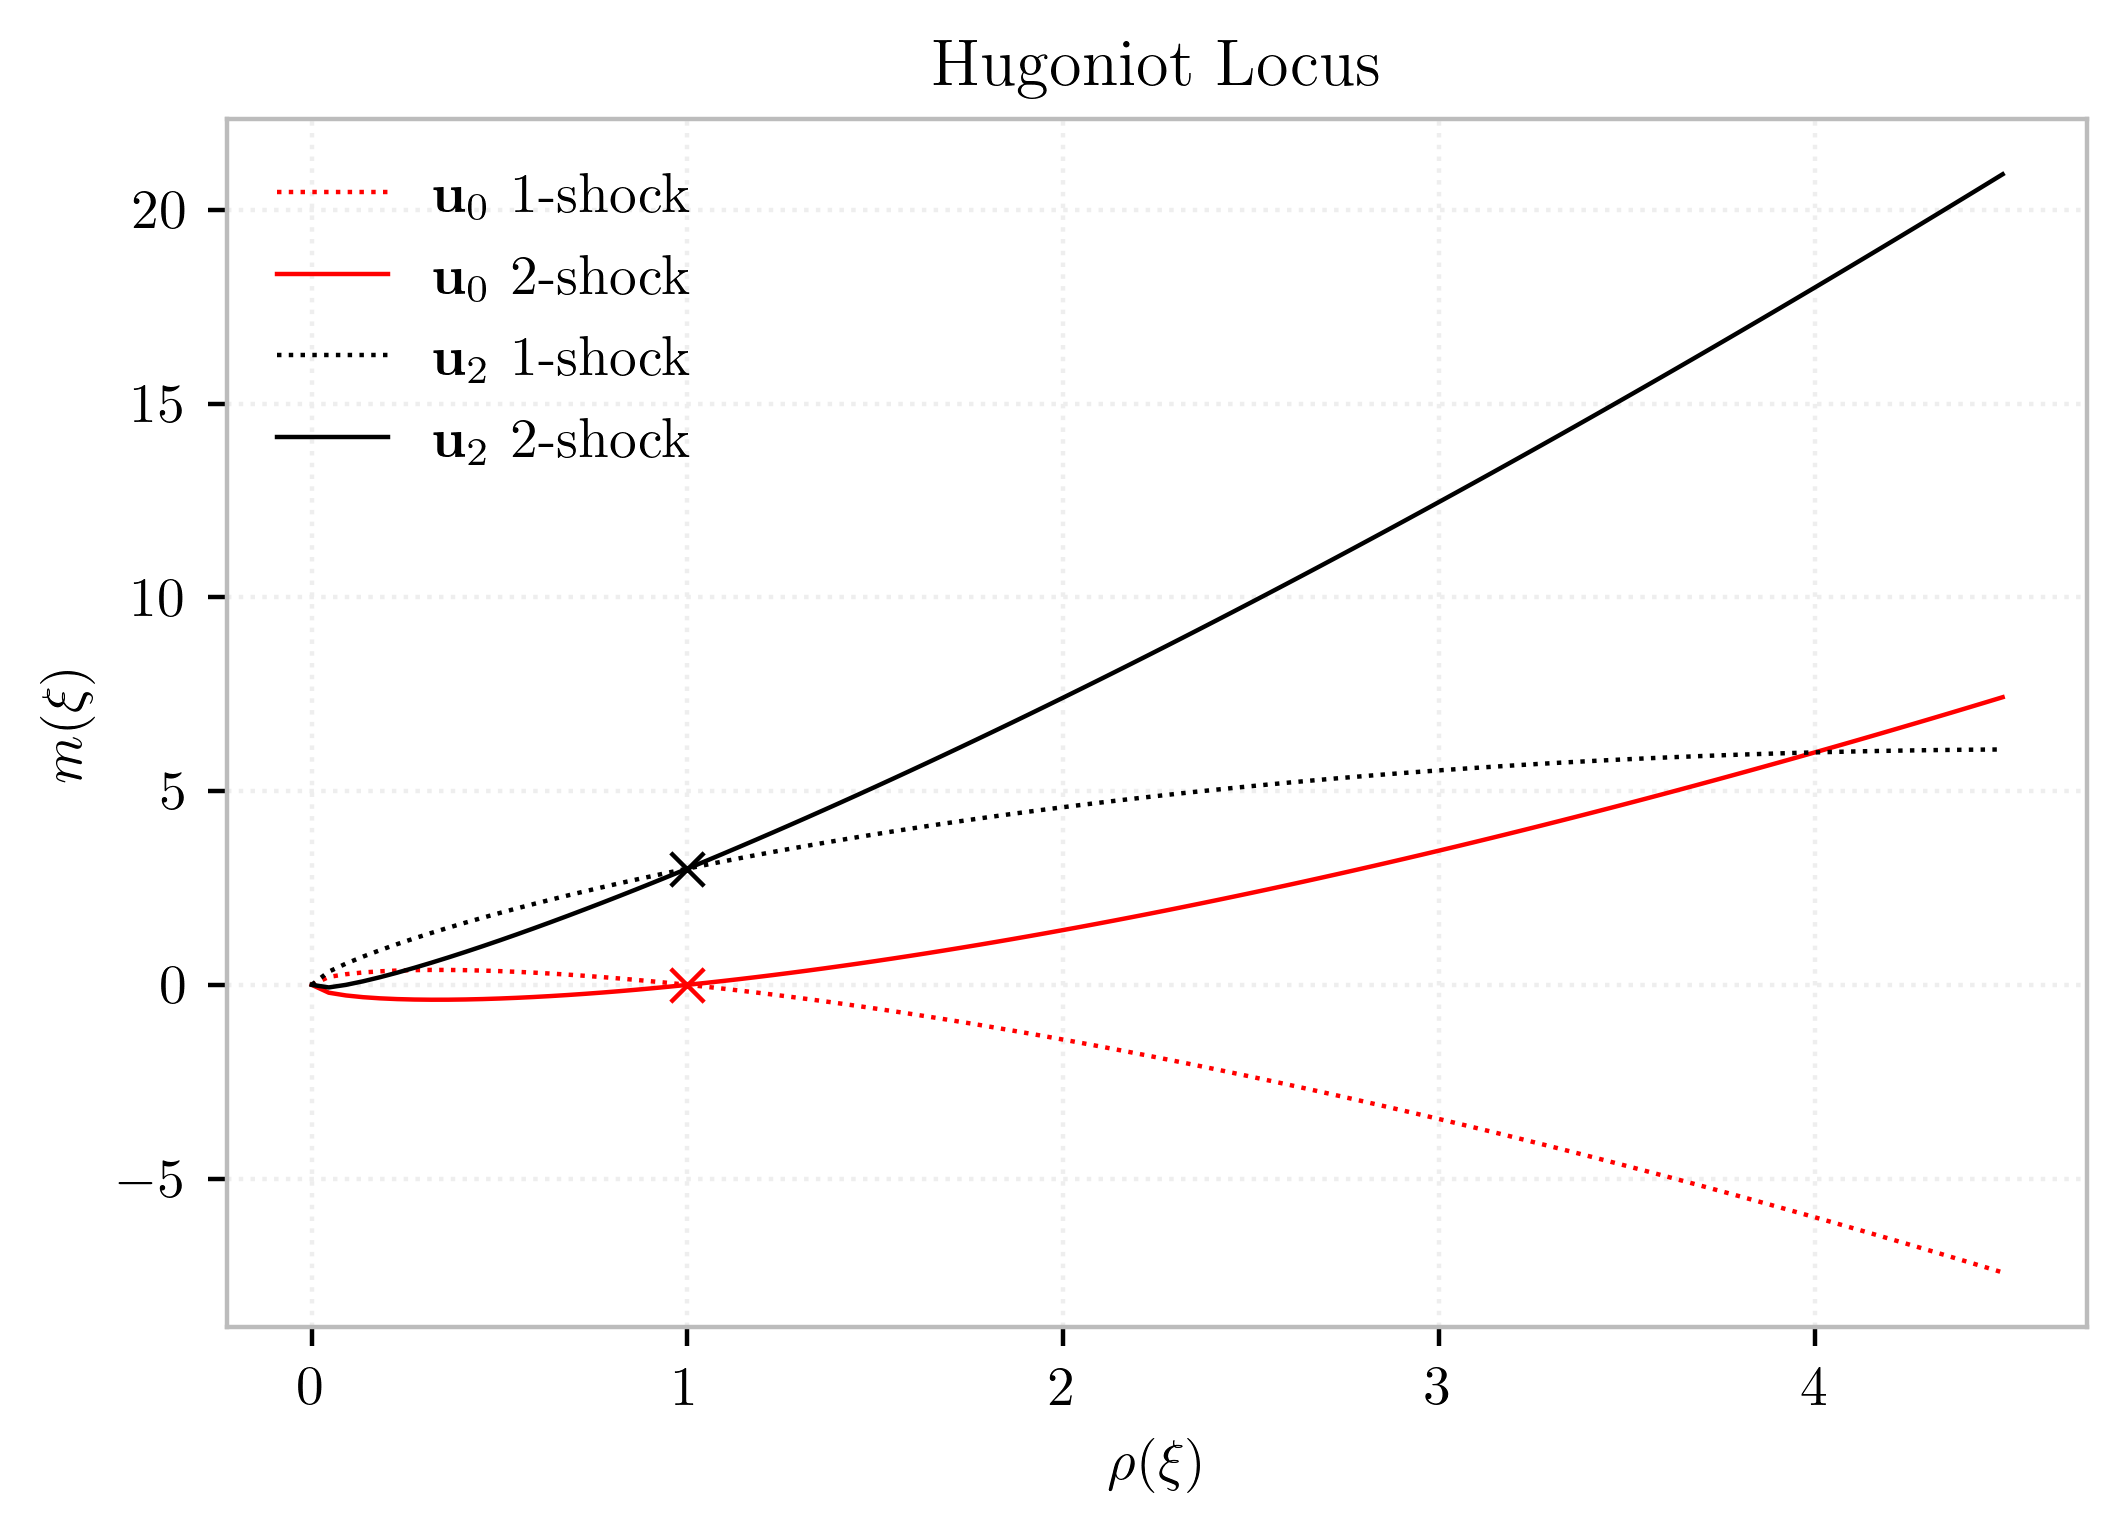
\includegraphics{../img/p1-locus.png}
\caption{Graphical solution of the isothermal Riemann problem}
\end{figure}

\[
\rho_{1} m_{0} / \rho_{0}-a \sqrt{\rho_{1} / \rho_{0}}\left(\rho_{1}-\rho_{0}\right)=\rho_{1} m_{2} / \rho_{2}+a \sqrt{\rho_{1} / \rho_{2}}\left(\rho_{1}-\rho_{2}\right)
\]

\[
\left(\frac{a}{\sqrt{\rho_{2}}}+\frac{a}{\sqrt{\rho_{0}}}\right) z^{2}+\left(\frac{m_{2}}{\rho_{2}}-\frac{m_{0}}{\rho_{0}}\right) z-a\left(\sqrt{\rho_{2}}+\sqrt{\rho_{0}}\right)=0
\]

Plugging in the specified values for \(q_0\) and \(q_2\) yields the
following coefficients:

\[
\begin{aligned}
\frac{a}{\sqrt{\rho_{2}}}+\frac{a}{\sqrt{\rho_{0}}} = 2\\
\frac{m_{2}}{\rho_{2}}-\frac{m_{0}}{\rho_{0}} = -3\\
a\left(\sqrt{\rho_{2}}+\sqrt{\rho_{0}}\right) = -2
\end{aligned}
\]

This yields the following roots:

\[
\rho_1 = \left\{\frac{1}{4}, 4\right\} \\
\]

\[
m_1 =\rho_{m} m_{r} / \rho_{r}+a \sqrt{\rho_{m} / \rho_{r}}\left(\rho_{m}-\rho_{r}\right) \\
\]

\[
\boxed{q_1 = \begin{pmatrix}4 \\ 6\end{pmatrix}}
\]

\begin{quote}
In each region \(i=0,1,2\), compute the characteristic speeds, which are
the eigenvalues \(\lambda_{i1}\) and \(\lambda_{i2}\) of the Jacobian
\(J_i=DF(q_i)\). Also compute the fluid velocities \(v_i\).
\end{quote}

\[
DF(q_i)=\begin{pmatrix}
0 & 1 \\
a^{2}-m_i^{2} / \rho_i^{2} & 2 m_i / \rho_i
\end{pmatrix}
\]

\hypertarget{state-i0}{%
\subsubsection{\texorpdfstring{State
\(i=0\)}{State i=0}}\label{state-i0}}

\[
DF(q_0) = \begin{pmatrix}0 & 1\\ -8 & 6\end{pmatrix}
\]

\[
\lambda = \{2,4\}
\]

\[
\mathbf{Q} = \begin{pmatrix}
-0.4472136 & -0.24253563\\
-0.89442719 & -0.9701425 
\end{pmatrix}
\]

\[
v_0 = 3
\]

\hypertarget{state-i1}{%
\subsubsection{\texorpdfstring{State
\(i=1\)}{State i=1}}\label{state-i1}}

\[
\lambda_1 = \{1/2, 5/2\}
\]

\[
\mathbf{Q} = \begin{pmatrix}
-0.89442719& -0.37139068 \\
-0.4472136 & -0.92847669
\end{pmatrix}
\]

\[
v_1 = 3/2
\]

\[
\dot s_1 = 1
\]

\hypertarget{state-i2}{%
\subsubsection{\texorpdfstring{State
\(i=2\)}{State i=2}}\label{state-i2}}

\[
DF(q_2) = \begin{pmatrix} 0 & 1 \\ 1 & 0 \end{pmatrix}
\]

\[
\lambda_2 = (1,-1)
\]

\[
\mathbf{Q} = \frac{1}{\sqrt{2}}\begin{pmatrix}1 & -1 \\ 1 & 1\end{pmatrix}
\]

\[
v_2 = 0
\]

\[
\dot s_2 = 2
\]

\begin{quote}
Confirm that \(\lambda_{01}>\dot s_1>\lambda_{11}\) and
\(\lambda_{12}>\dot s_2>\lambda_{22}\), which are Lax's entropy
conditions for this system. Also confirm that \(v_0>\dot s_1\),
\(v_1>\dot s_1\), \(\dot s_2>v_1\) and \(\dot s_2>v_2\), which means
fluid particles move from the original states \(q_0\) and \(q_2\) to the
auxiliary state \(q_1\) as the shocks propagate through space and time.
\end{quote}

\newpage{}

\hypertarget{problem-3--alpha-u_xx-au-f}{%
\section{\texorpdfstring{Problem 3
(\(-\alpha u_{xx} + Au = f\))}{Problem 3 (-\textbackslash alpha u\_\{xx\} + Au = f)}}\label{problem-3--alpha-u_xx-au-f}}

\begin{quote}
Write a 1d finite element code to solve the modified Poisson equation \[
-\alpha u_{xx} + Au = f, \quad (0\le x\le 1), \qquad u(0)=0,\; u(1)=0,
\] where \(\alpha>0\) and \(A\ge0\). Use 4th order finite elments on a
uniformly spaced grid,

\[
x_j = j/M, \qquad\quad 0\le j\le M
\]

where \(M\) is divisible by 4 and the \(r\)th element includes nodes
\(x_{4r+i}\) for \(0\le r<M/4\) and \(0\le i\le 4\).
\end{quote}

\hypertarget{part-a}{%
\subsection{Part A}\label{part-a}}

Multiplying by a test function \(v\) and integrating over the domain
(applying integration by parts) yields:

\[
\int_\Omega -\alpha u_{xx} v + \gamma u v = \int_\Omega f v
\]

\[
\int \alpha u_x v_x dx - \left. \alpha u_x v \right| + \gamma \int u v dx = \int f v dx
\]

For test functions which vanish on the boundary one obtains:

\[
\int_\Omega \alpha u_x v_x + \gamma u v = \int_\Omega f v
\]

\[
a(\alpha u,v) + \langle Au,v \rangle = \langle f,v\rangle
\]

\hypertarget{fourth-order-element}{%
\subsubsection{Fourth-order element}\label{fourth-order-element}}

A fourth order isoparametric 1D element is developed by applying
Lagrange interpolation over 5 equally spaced sampling points.

\begin{figure}
\centering
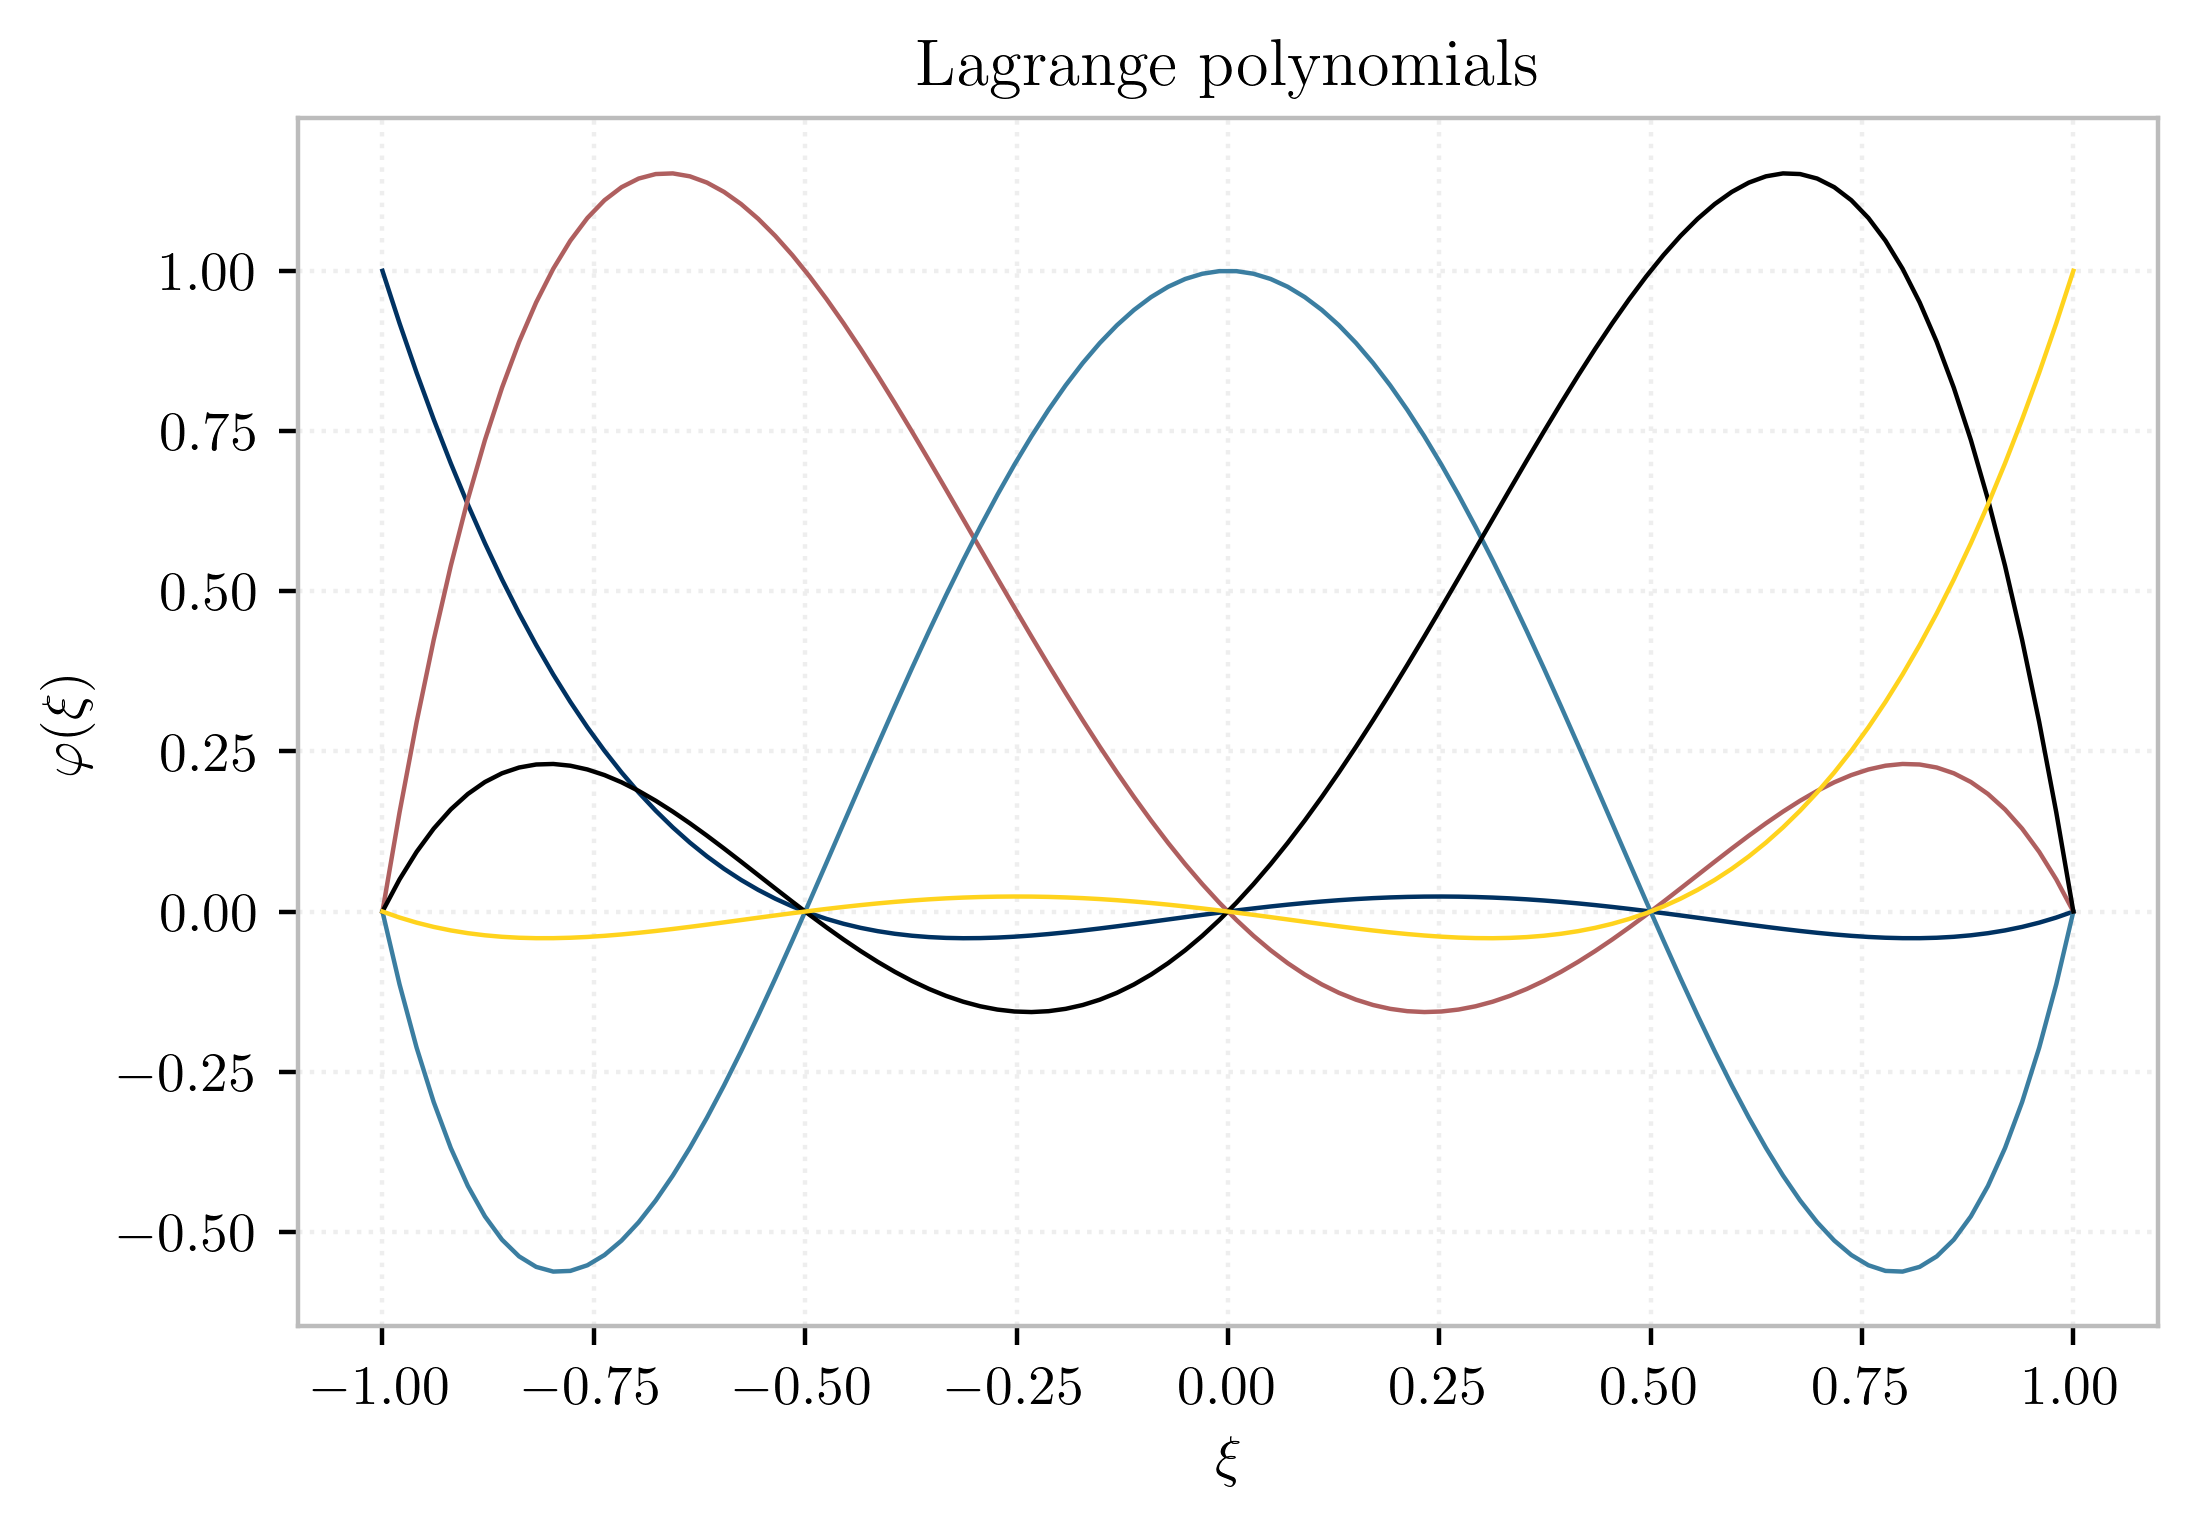
\includegraphics{../img/lagrange.png}
\caption{Shape functions}
\end{figure}

\hypertarget{convergence}{%
\subsubsection{Convergence}\label{convergence}}

\begin{quote}
\begin{enumerate}
\def\labelenumi{(\alph{enumi})}
\tightlist
\item
  Do a convergence study for \(\alpha=1/100\), \(A=0\) and
  \(f(x)=\frac{\pi^2}{100}\sum_{k=0}^4 \sin\big((2k+1)\pi x \big)\).
\end{enumerate}
\end{quote}

The exact integral for this problem is as follows:

\[
\frac{1}{\alpha 100} \sum{\frac{1}{(2k+1)^2}\sin{\left((2k+1)\pi x\right)} }
\]

\begin{figure}
\centering
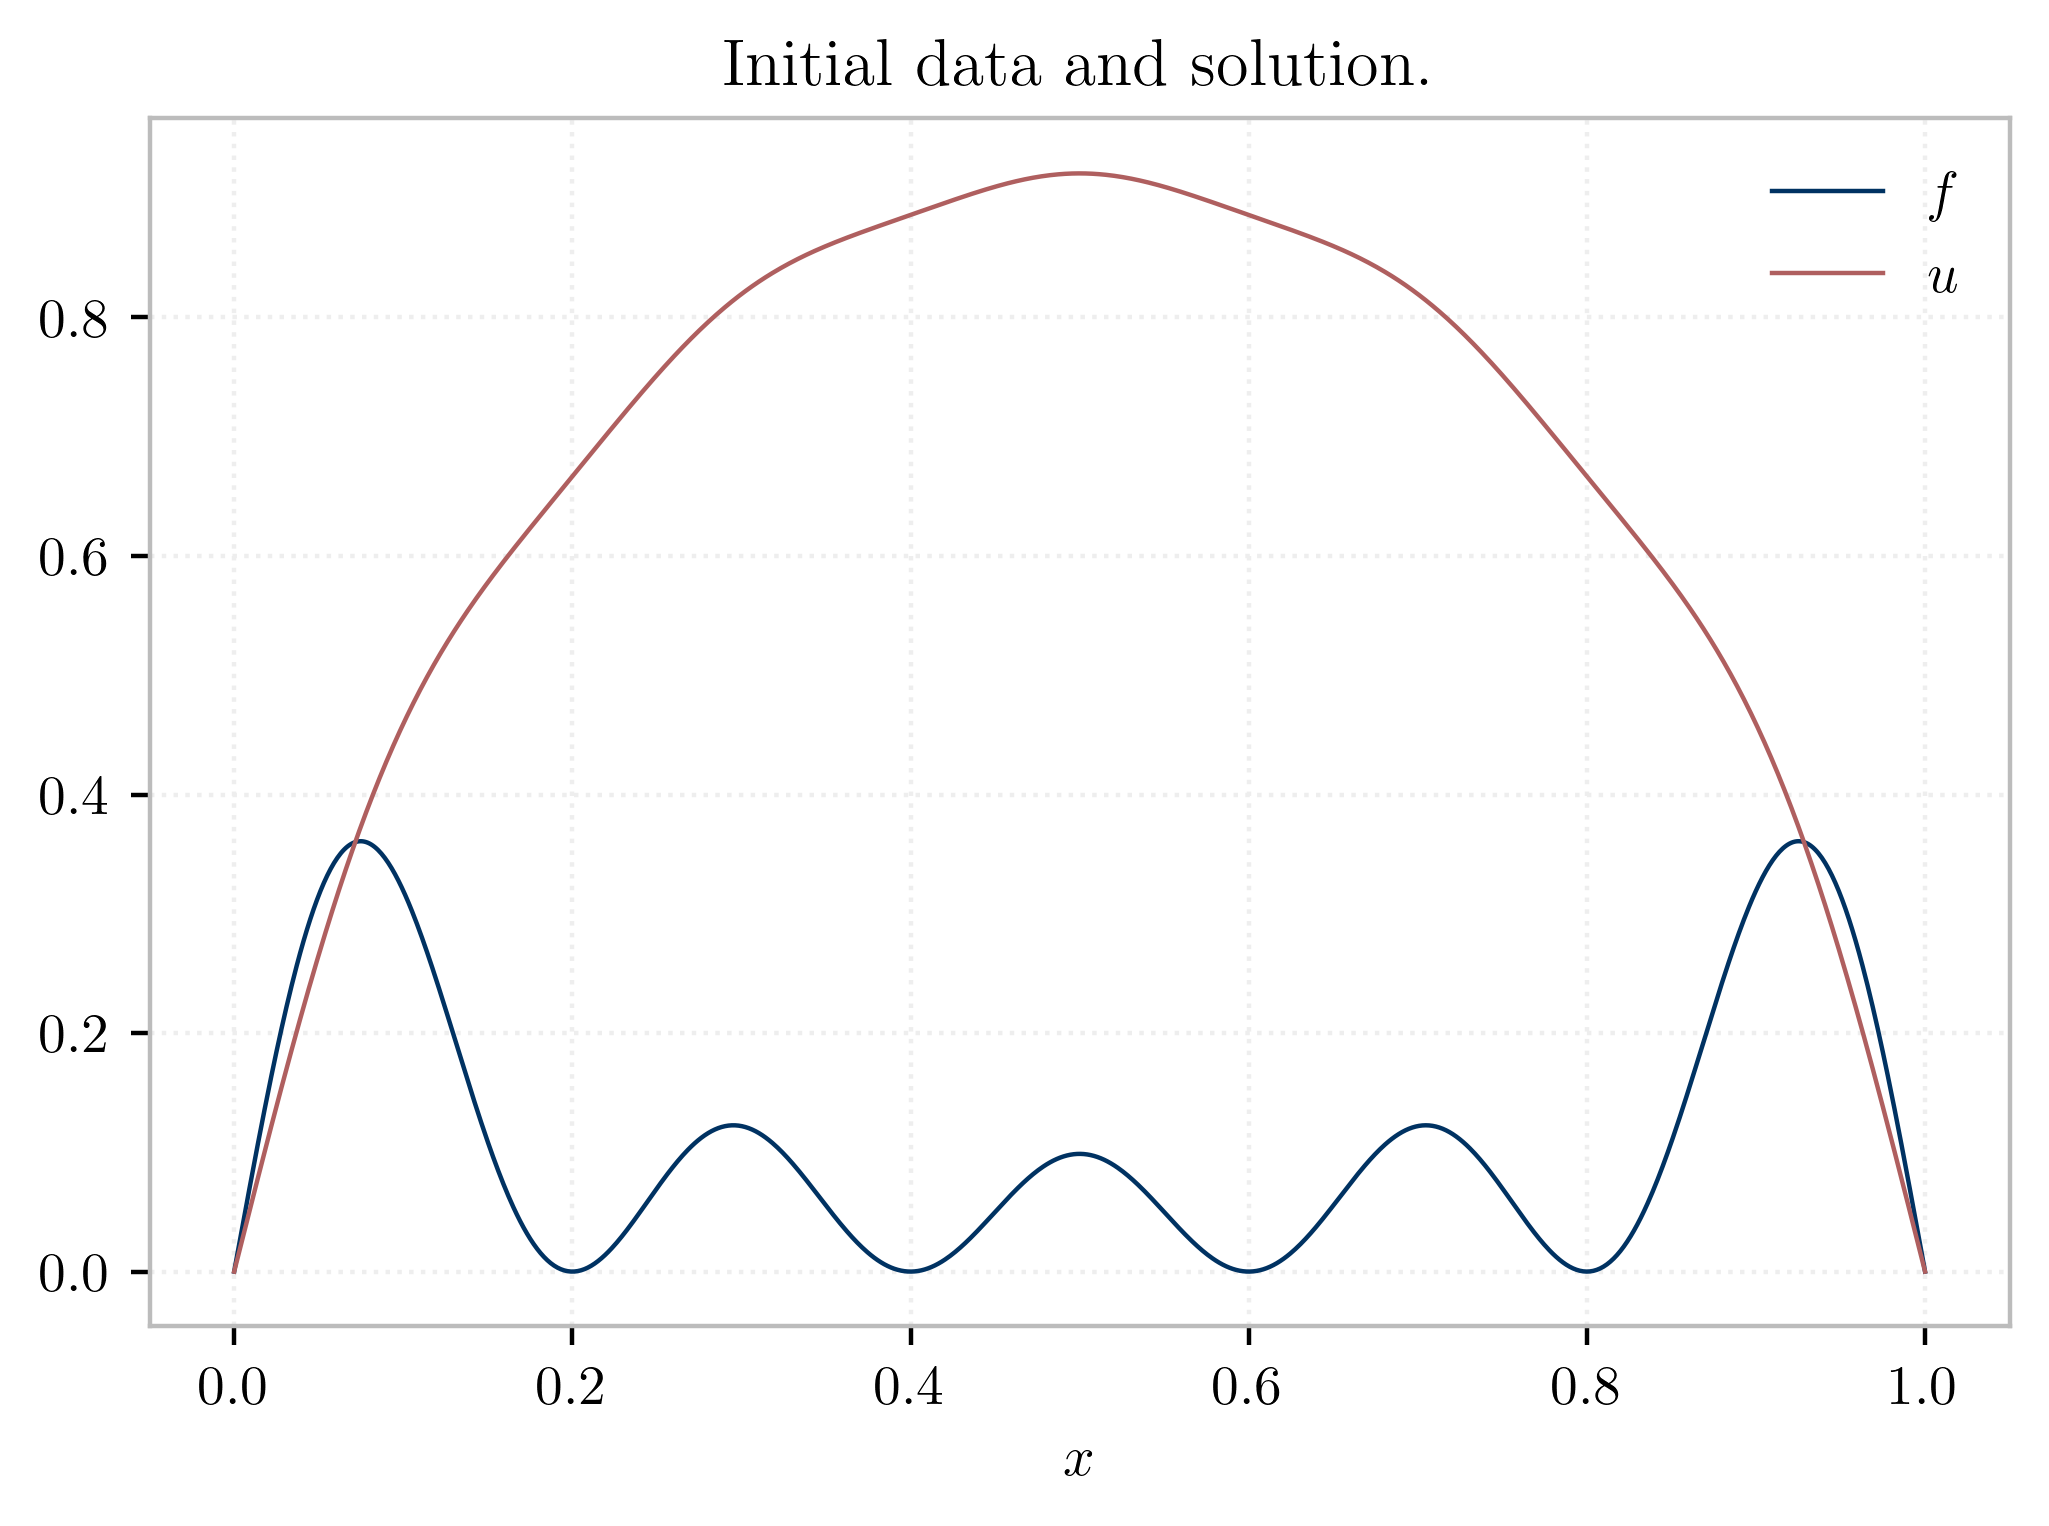
\includegraphics{../img/p3a-exact.png}
\caption{Source curve \(f\) and exact solution \(u\)}
\end{figure}

\begin{figure}
\centering
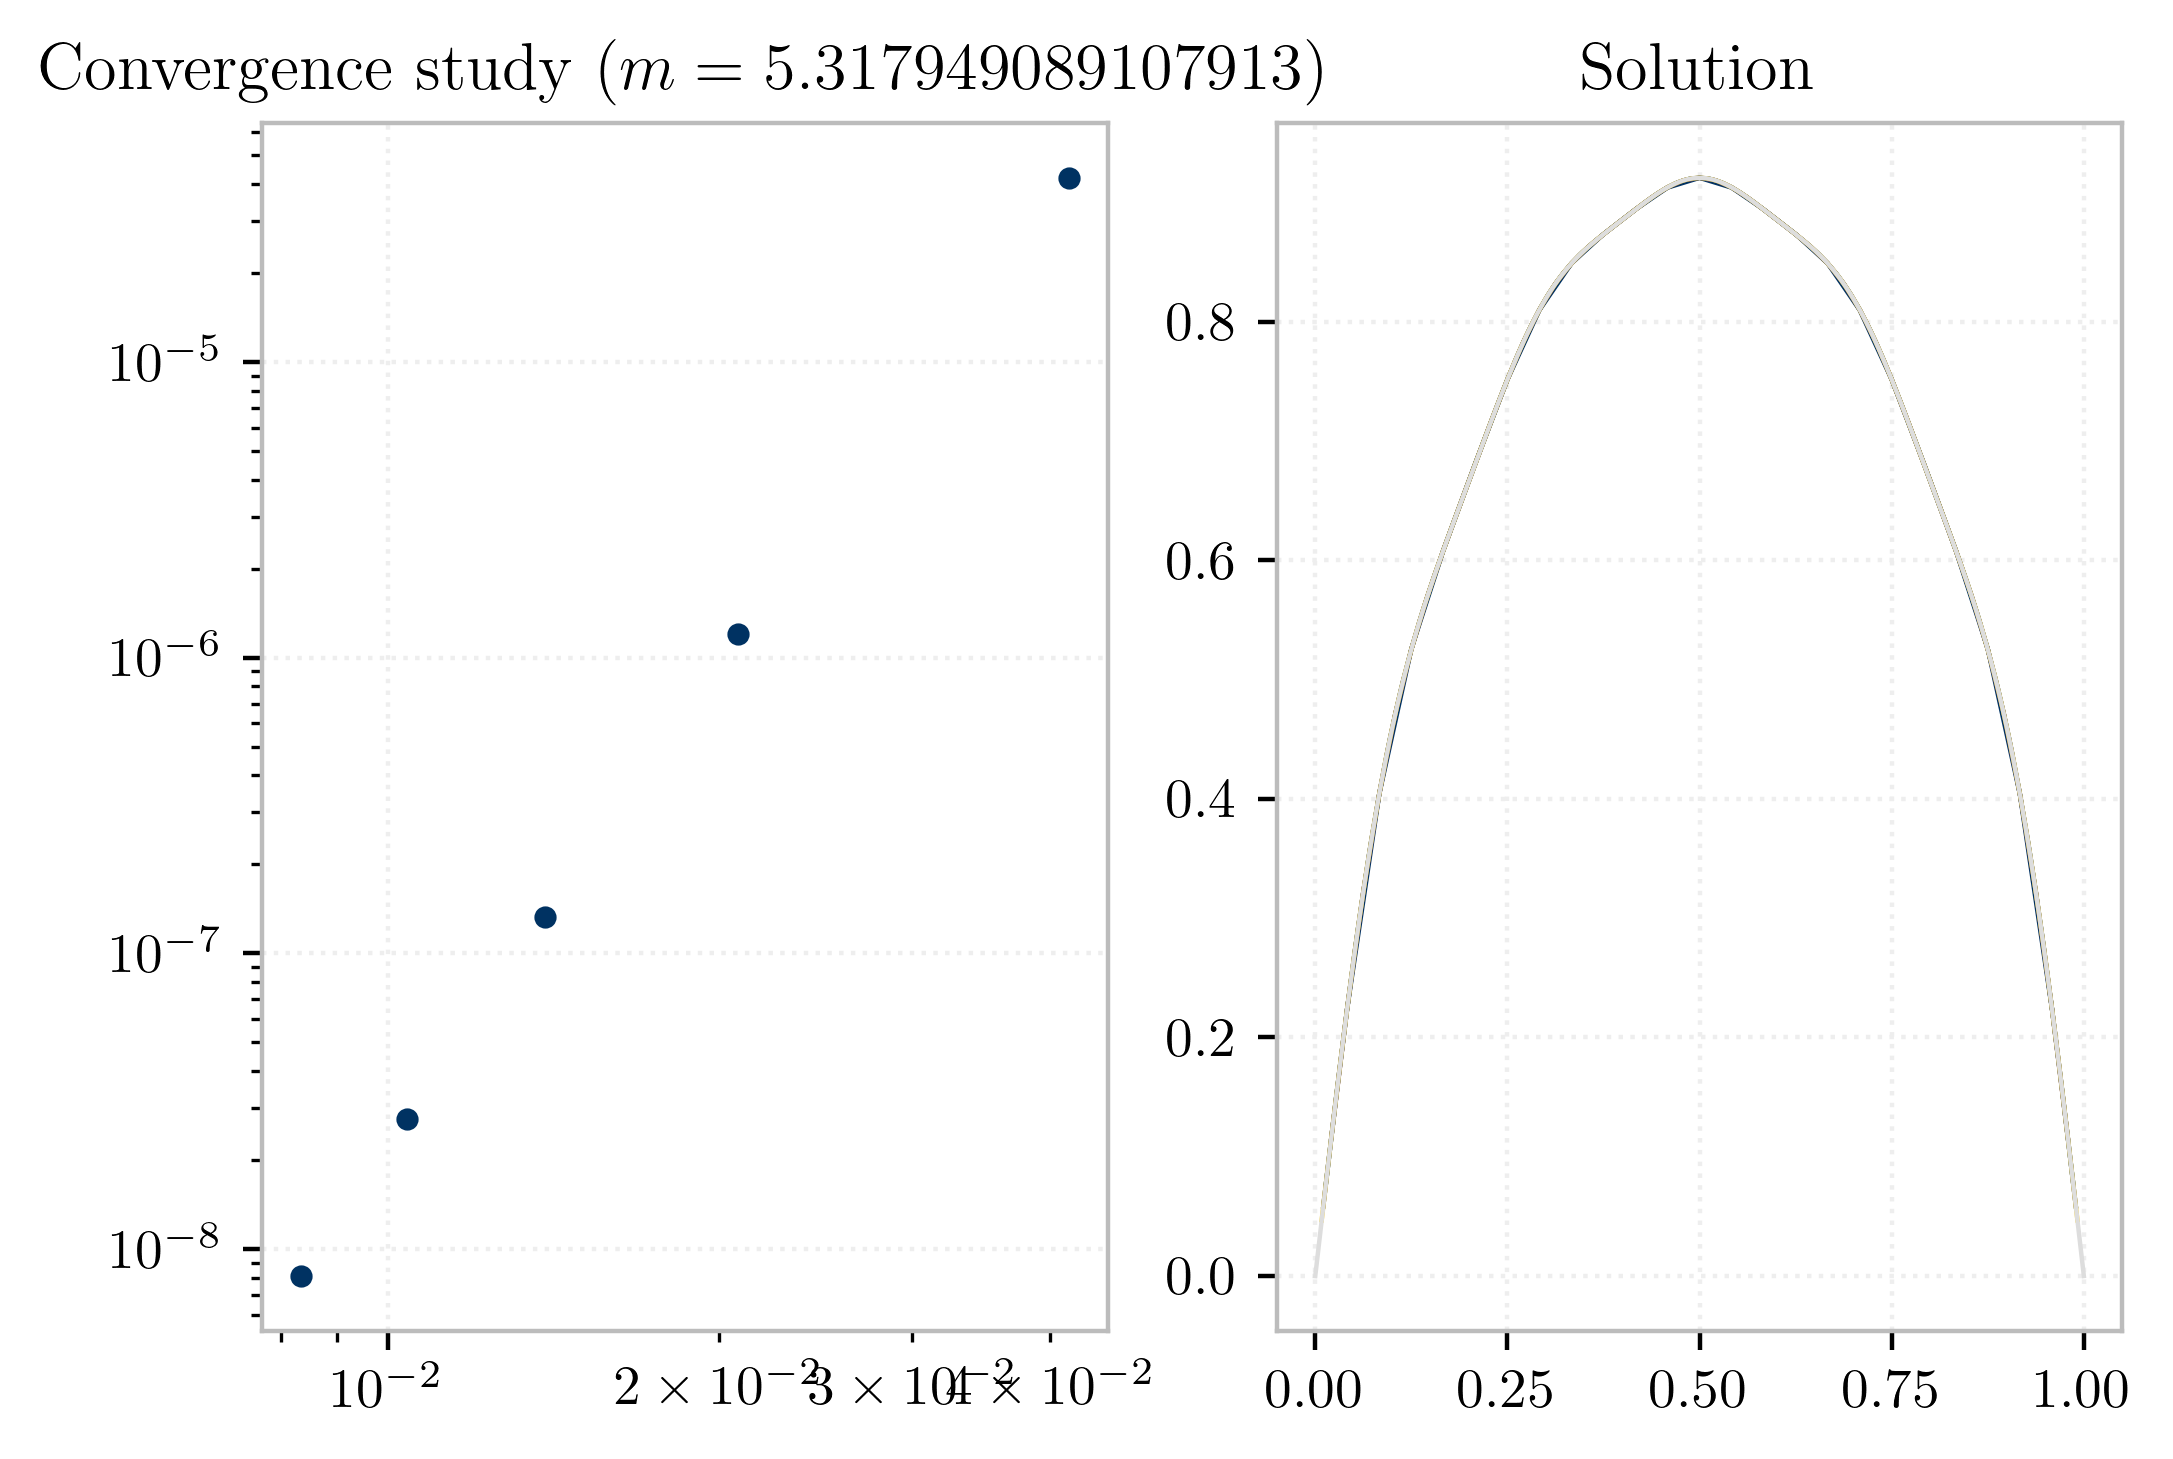
\includegraphics{../img/p3a-conv.png}
\caption{Convergence study for finite element solution of steady-state
problem.}
\end{figure}

\newpage{}

\hypertarget{part-b-transient-analysis}{%
\subsection{Part B: Transient
Analysis}\label{part-b-transient-analysis}}

\begin{quote}
\begin{enumerate}
\def\labelenumi{(\alph{enumi})}
\setcounter{enumi}{1}
\tightlist
\item
  Solve \(u_t=\frac1{100}u_{xx}+f(x)\sin(\pi t)\) from \(t=0\) to
  \(t=1\) with initial condition \(u(x,0)=0\) and the same \(f\) as in
  part (a). Use the 4th order implicit SDIRK timestepper with Butcher
  array given in problem 2 of HW 2. Use your finite element code above
  to solve the implicit equation for each stage of the timestepper.
  (I'll explain this in class). Make a convergence plot for several
  values of \(M\) and one choice of \(\nu=k/h\) that you find works
  well.
\end{enumerate}
\end{quote}

The exact solution of the transient problem was derrived using the
\texttt{sympy} CAS library. A plot is shown below for various times.

\begin{figure}
\centering
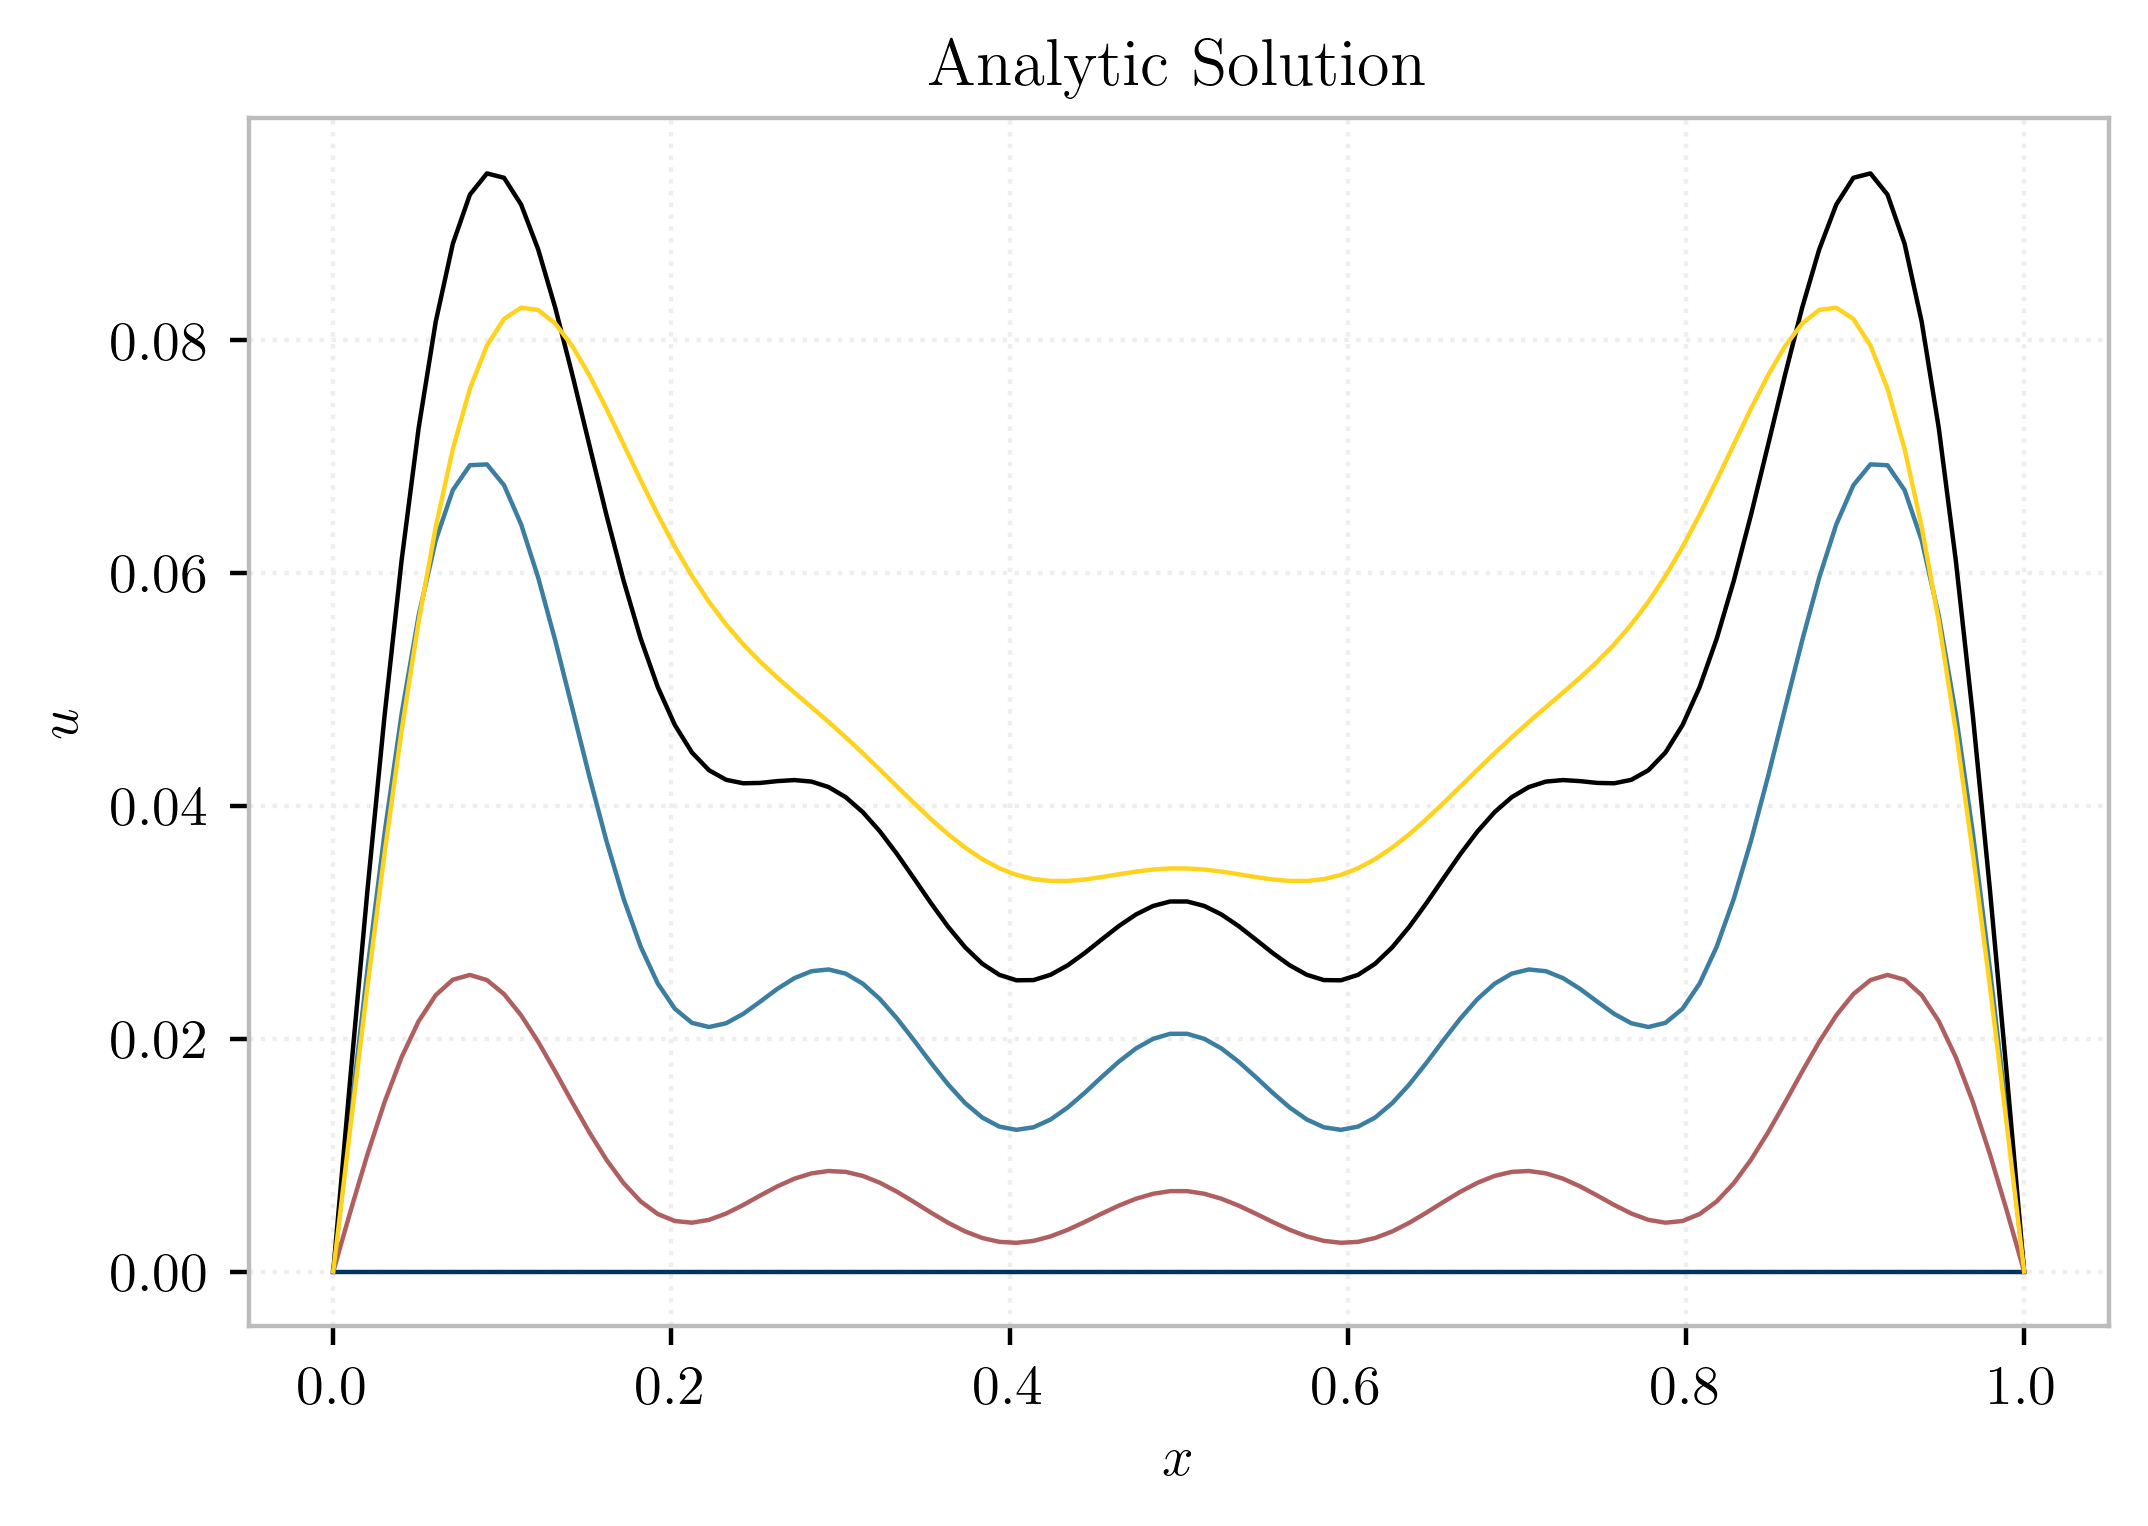
\includegraphics{../img/p3b-exact.png}
\caption{Analytic solution curves}
\end{figure}

\begin{figure}
\centering
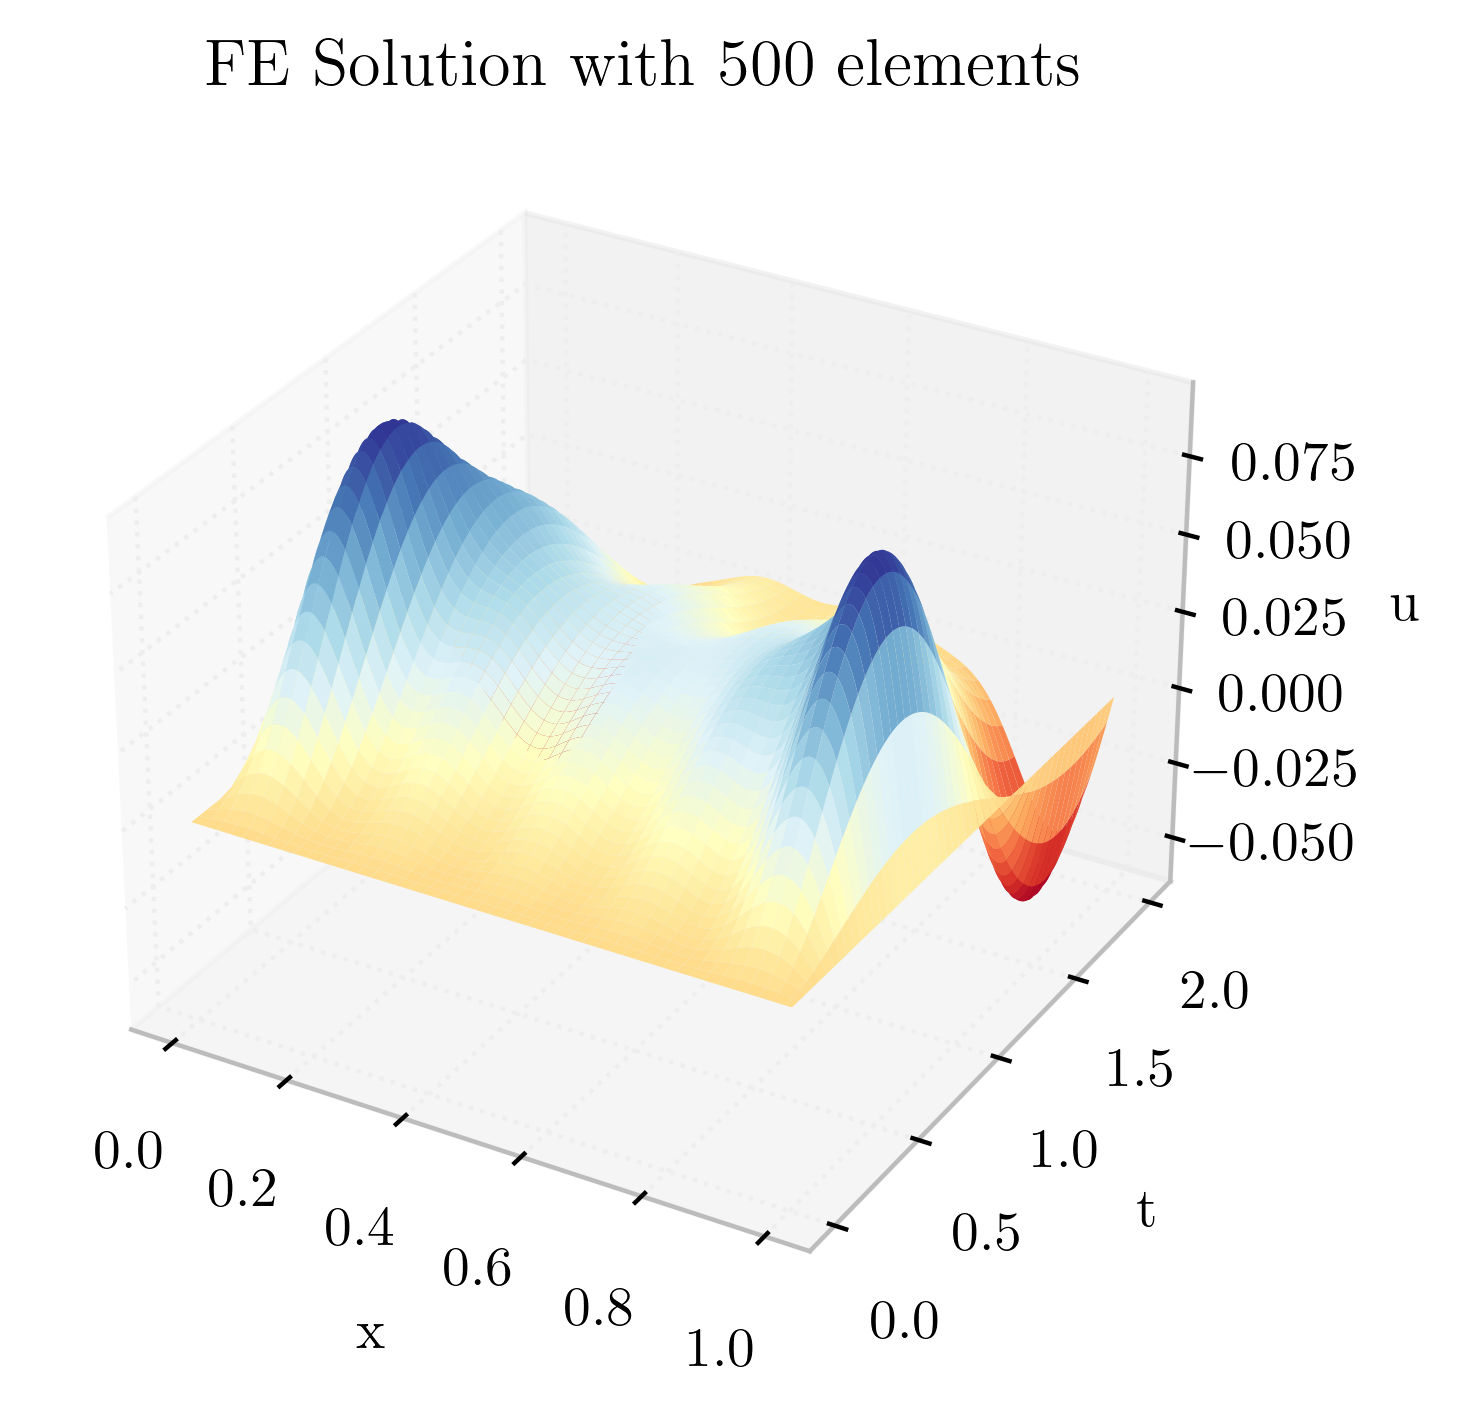
\includegraphics{../img/p3b-fem-iso.png}
\caption{FEM solution}
\end{figure}

\hypertarget{sdirk-implementation}{%
\subsubsection{SDIRK Implementation}\label{sdirk-implementation}}

In HW2 a Runge-Kutta algorithm was implemented for problems with the
following form:

\[
\mathbf{u}_t + B\mathbf{u} = \mathbf{d}(t)
\]

Where \(B\) is a linear operator . At stage \(i\) of a diagonal
Runge-Kutta method one has

\[
\ell_{i}=F\left(t_{n}+c_{i} k, \vec{u}_{n}+k \sum_{j=1}^{i-1} a_{i j} \ell_{j}+k a_{i j} \ell_{i}\right)
\]

where \(k=\Delta t\). For problems of the aforementioned form, this
simplifies to

\[
\left(I - k a_{i i} B\right) \ell_{i} = B \left(\vec{u}_{n}+k \sum_{j=1}^{i-1} a_{i j} \ell_{j}\right) + d(t_n+c_i k) 
\]

The following data is required to set up a particular scheme for
\(\mathbf{u}\in \mathbb{R}^n\) with \(s\in\mathbf{Z^+}\) stages:

\begin{description}
\tightlist
\item[\(\mathcal{T}\)]
A Butcher tableau with zero entries above the diagonal.
\end{description}

\(B, \mathbb{R}^n \rightarrow \mathbb{R}^n\): Discrete space operator

\begin{description}
\tightlist
\item[\(\mathbf{d}, \mathbb{R} \rightarrow \mathbb{R}^n\)]
Source term.
\end{description}

The problem at hand is manipulated to fit the following form:

\[\vec{u}_{t}=-\frac{1}{100} {M}^{-1} A \vec{u}+\vec{f} \sin \pi t\]

so that

\[
\begin{gathered}
B=\frac{-1}{100}M^{-1}A \\
\mathbf{d}=M^{-1}b\sin{\pi t}
\end{gathered}
\]

where \(A\), \(M\), and \(b\) are the stiffness, mass and load vectors
as readily produced by the implementation for Part B.

\[
\left(M+\frac{k a_{i i}}{100} A\right) l_{i} = -\frac{1}{100} A\left(\vec{u}_{n}+k \sum_{j=1}^{i-1} a_{i j} \ell_{j}\right) + M \vec{f} \sin \pi\left(t_{n}+c_{i} k\right)
\]

The tableau \(\mathcal{T}\) is given as

\[
\begin{array}{c|ccccc}
  1/4 & 1/4 \\
  3/4 & 1/2 & 1/4 \\
  11/20 & 17/50 & -1/25 & 1/4 \\
  1/2 & 371/1360 & -137/2720 & 15/544 & 1/4 \\
  1 & 25/24 & -49/48 & 125/16 & -85/12 & 1/4 \\
  \hline
  & 25/24 & -49/48 & 125/16 & -85/12 & 1/4
\end{array}
\]

\begin{center}\rule{0.5\linewidth}{0.5pt}\end{center}

\(u(x,t) = \sum_j u_j(t)\phi_j(x)\)

\[u_{t}=\frac{1}{100} u_{x x}+f(x) \sin \pi t\]

let \(u_t = \sum_ju_{j,t}\phi_j\), and \(v=\phi_i\)

\[
\langle u_{t}, v\rangle = -\frac{1}{100} a(u, v)+\langle f, v\rangle \sin \pi t
\]

\[
M \vec{u}_{t}=-\frac{1}{100} A \vec{u} + M \vec{f} \sin \pi t
\]

\[
\vec{u}_{t}=-\frac{1}{100} {M}^{-1} A \vec{u}+\vec{f} \sin \pi t
\]

\hypertarget{convergence-1}{%
\subsubsection{Convergence}\label{convergence-1}}

Convergence studies are presented below for time discretizations using
both the SDIRK scheme provided and the Crank-Nicolson scheme.

\begin{figure}
\centering
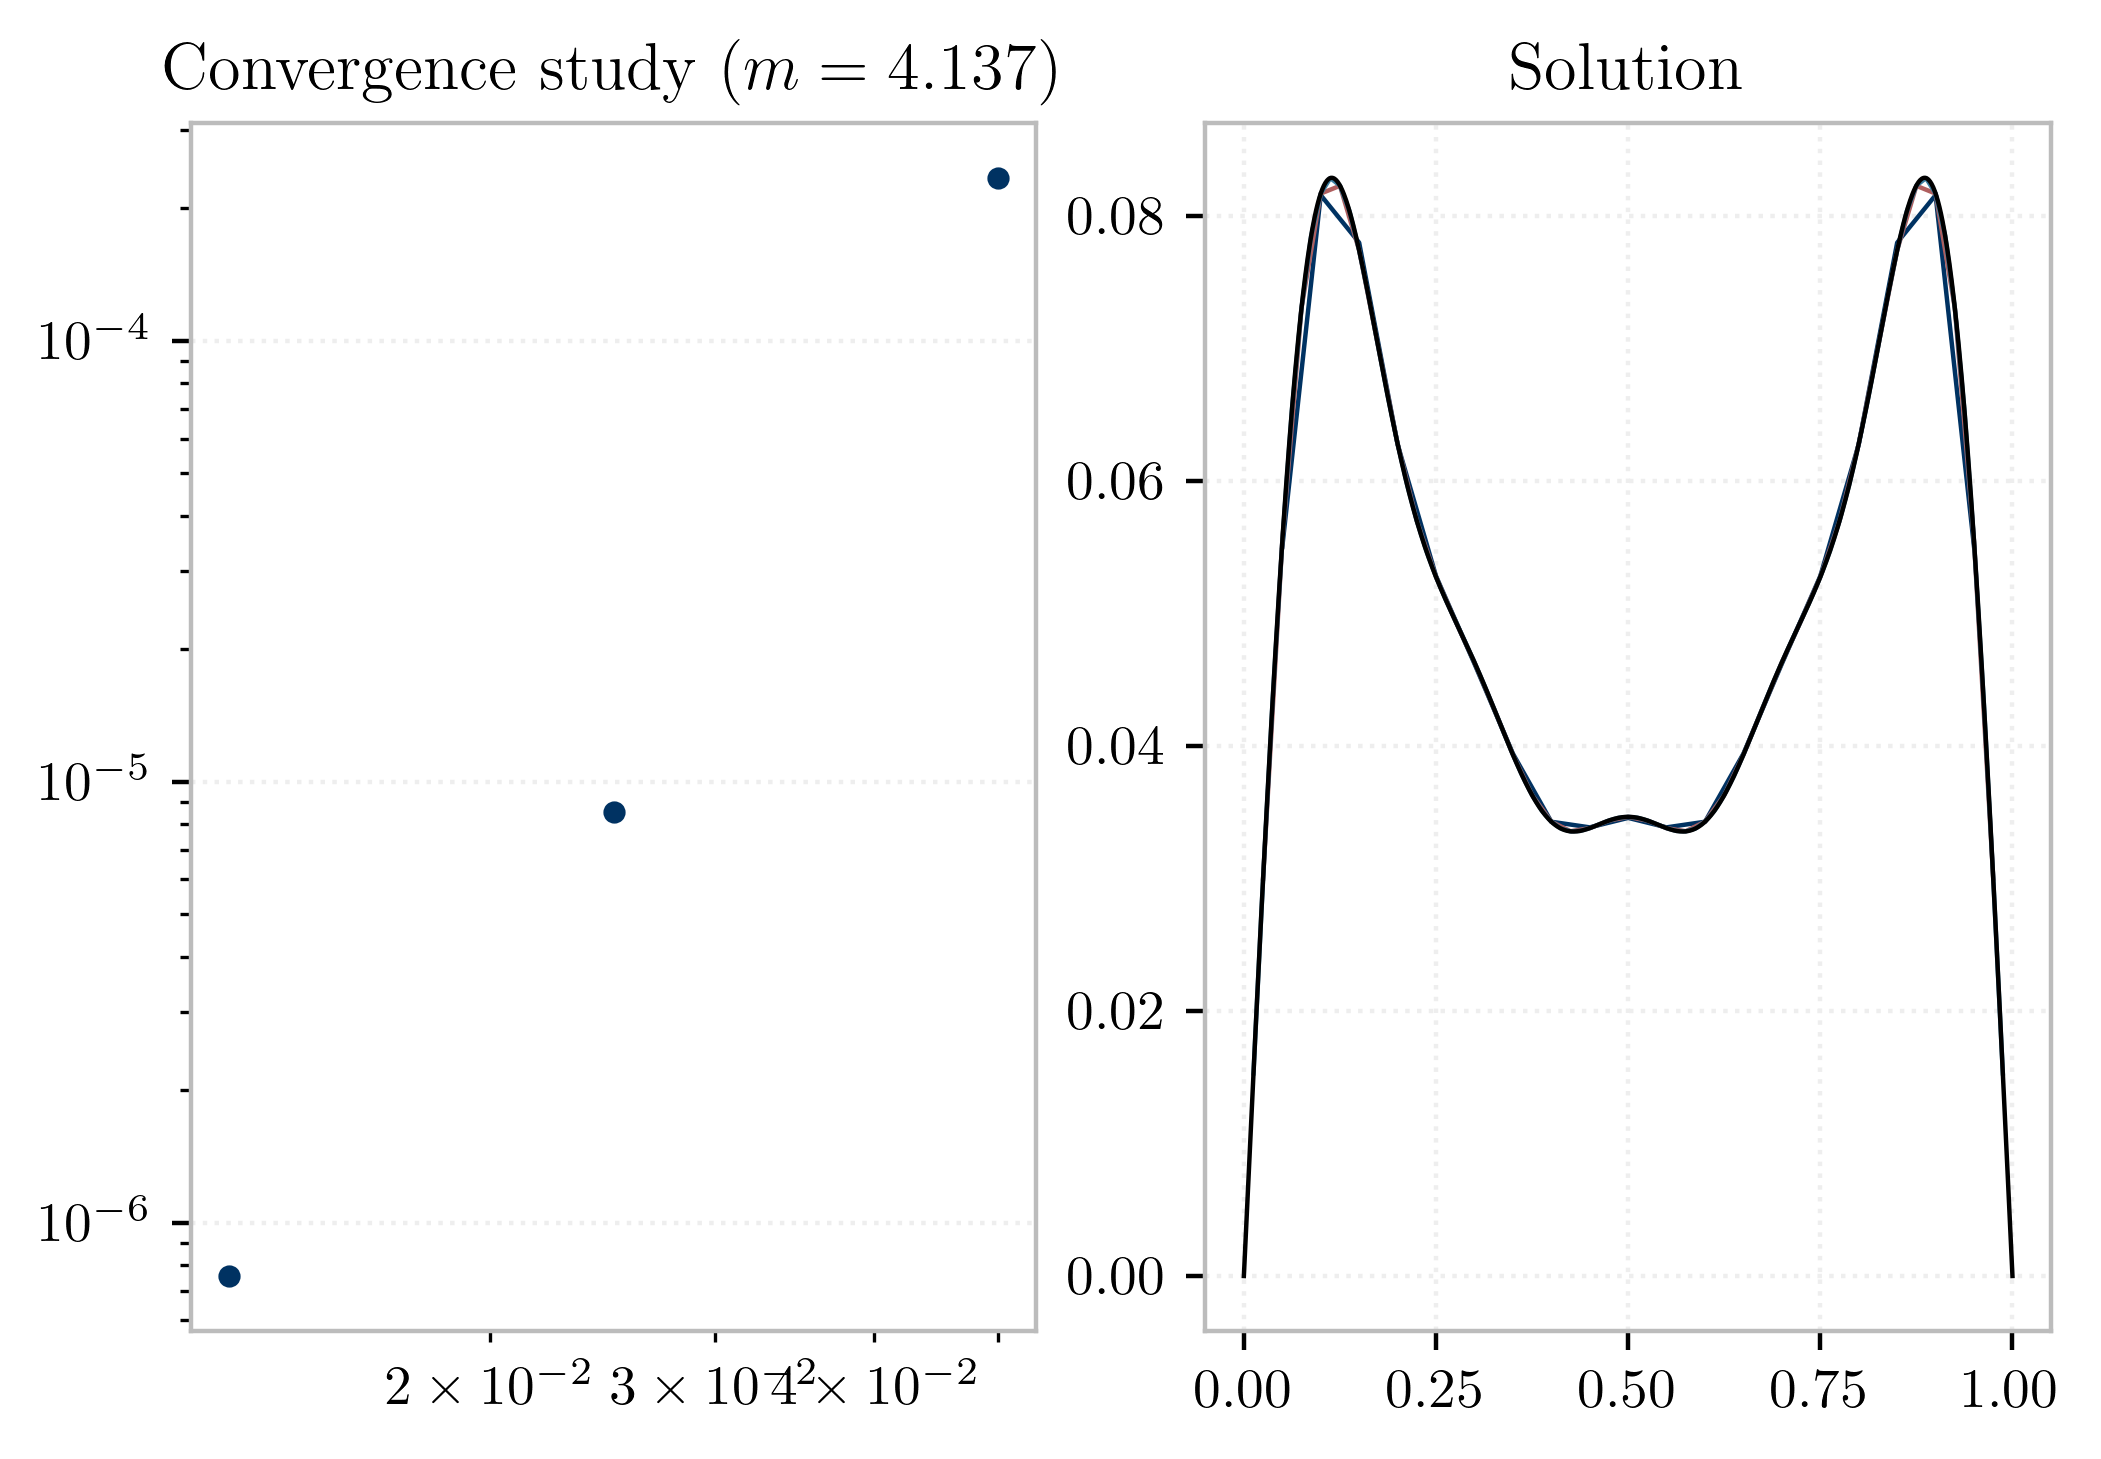
\includegraphics{../img/p3b-conv.png}
\caption{Convergence study.}
\end{figure}

\begin{figure}
\centering
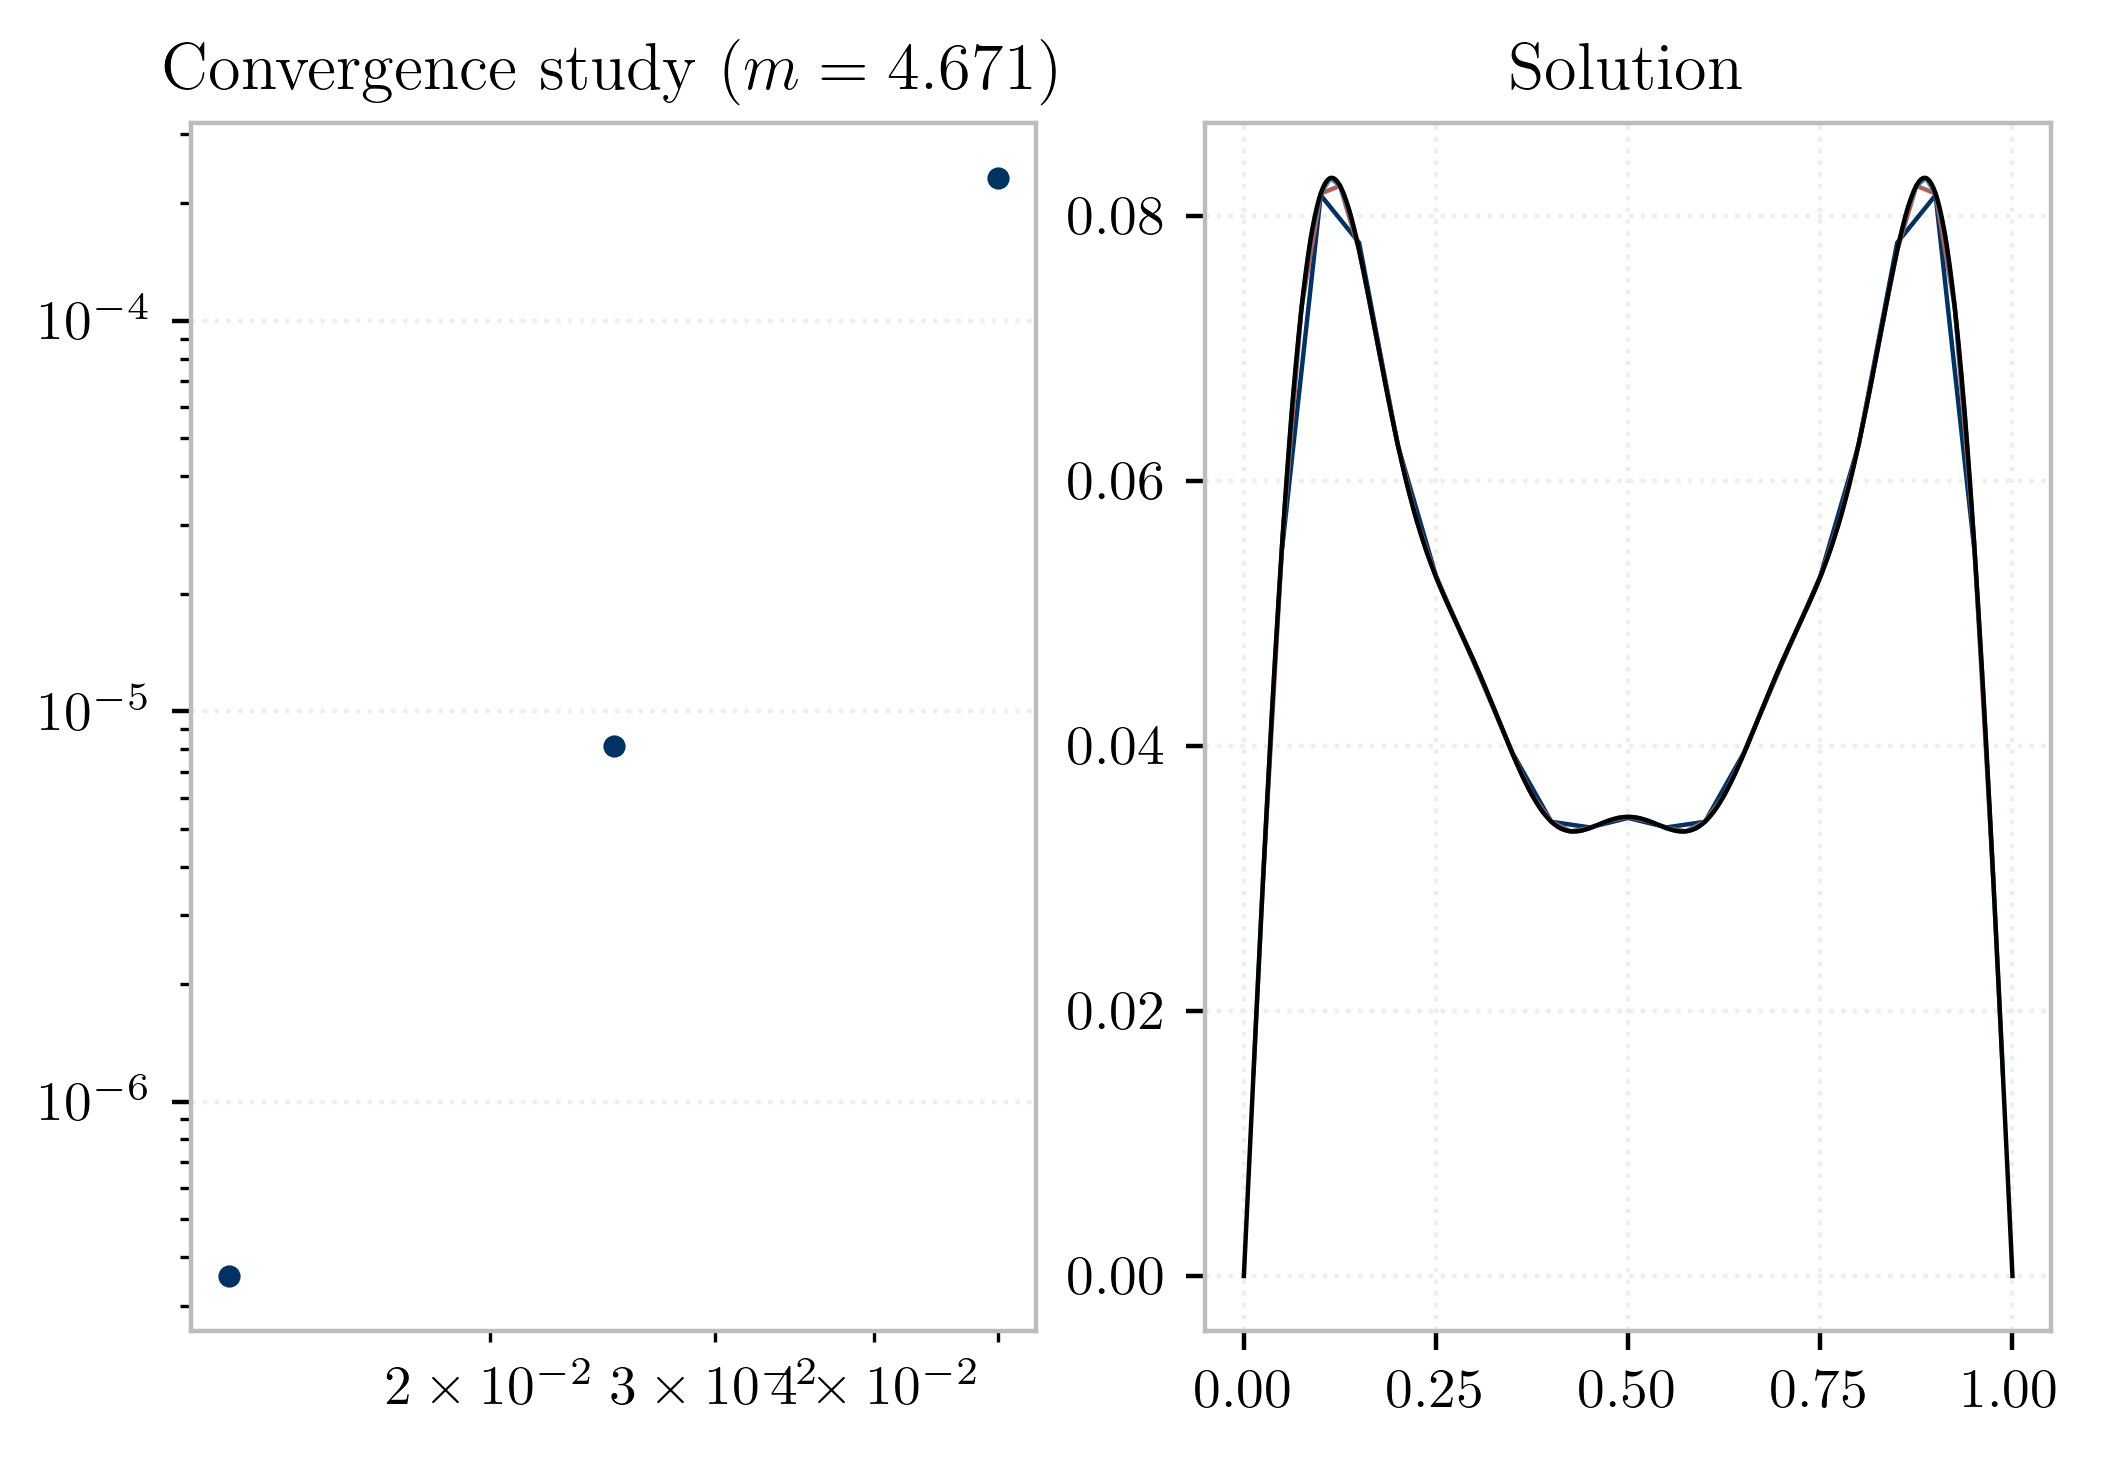
\includegraphics{../img/p3b-conv-cn.png}
\caption{Convergence study for Crank-Nicolson tableau.}
\end{figure}

\newpage{}

\hypertarget{appendix}{%
\section{Appendix}\label{appendix}}

Key source code excerpts are provided below. The Python libraries
\texttt{elle}, \texttt{emme}, \texttt{anon} and \texttt{m228} which have
been used throughout are self written and available either from
\url{PyPi.org} via \texttt{pip} or on Github.

\hypertarget{source-code}{%
\subsection{Source Code}\label{source-code}}

\hypertarget{fourth-order-lagrange-element}{%
\subsubsection{Fourth-order Lagrange
element}\label{fourth-order-lagrange-element}}

\begin{Shaded}
\begin{Highlighting}[]
\CommentTok{\# external imports}
\ImportTok{import}\NormalTok{ jax}
\CommentTok{\# internal imports}
\ImportTok{import}\NormalTok{ anon}
\ImportTok{import}\NormalTok{ anon.atom }\ImportTok{as}\NormalTok{ anp}
\ImportTok{from}\NormalTok{ anon }\ImportTok{import}\NormalTok{ quad}

\AttributeTok{@anon.dual.generator}\NormalTok{(}\DecValTok{5}\NormalTok{)}
\KeywordTok{def}\NormalTok{ elem\_0001(f}\OperatorTok{=}\VariableTok{None}\NormalTok{,a1}\OperatorTok{=}\FloatTok{1.0}\NormalTok{, a2}\OperatorTok{=}\FloatTok{0.0}\NormalTok{,order}\OperatorTok{=}\DecValTok{4}\NormalTok{):}
    \CommentTok{"""}
\CommentTok{    Fourth order 1D Lagrange finite element with uniformly spaced nodes.}
\CommentTok{    }
\CommentTok{    Parameters}
\CommentTok{    {-}{-}{-}{-}{-}{-}{-}{-}{-}{-}}
\CommentTok{    f: Callable}
\CommentTok{        element loading.}
\CommentTok{    a1: float}
\CommentTok{        Stiffness coefficient}
\CommentTok{    a2: float}
\CommentTok{        Mass coefficient}
\CommentTok{    """}
\NormalTok{    state }\OperatorTok{=}\NormalTok{ \{\}}
    \ControlFlowTok{if}\NormalTok{ f }\KeywordTok{is} \VariableTok{None}\NormalTok{: f }\OperatorTok{=} \KeywordTok{lambda}\NormalTok{ x: }\FloatTok{0.0}

    \KeywordTok{def}\NormalTok{ transf(xi: }\BuiltInTok{float}\NormalTok{,x\_nodes)}\OperatorTok{{-}\textgreater{}}\BuiltInTok{float}\NormalTok{:}
        \ControlFlowTok{return}\NormalTok{ ( x\_nodes[}\DecValTok{0}\NormalTok{]}\OperatorTok{*}\NormalTok{( }\OperatorTok{+}\NormalTok{ xi}\OperatorTok{/}\DecValTok{6}\NormalTok{) }
               \OperatorTok{+}\NormalTok{ x\_nodes[}\DecValTok{1}\NormalTok{]}\OperatorTok{*}\NormalTok{( }\OperatorTok{{-}} \DecValTok{4}\OperatorTok{*}\NormalTok{xi}\OperatorTok{/}\DecValTok{3}\NormalTok{) }
               \OperatorTok{+}\NormalTok{ x\_nodes[}\DecValTok{2}\NormalTok{]}\OperatorTok{*}\NormalTok{( }\OperatorTok{+} \DecValTok{1}\NormalTok{) }
               \OperatorTok{+}\NormalTok{ x\_nodes[}\DecValTok{3}\NormalTok{]}\OperatorTok{*}\NormalTok{( }\OperatorTok{+} \DecValTok{4}\OperatorTok{*}\NormalTok{xi}\OperatorTok{/}\DecValTok{3}\NormalTok{) }
               \OperatorTok{+}\NormalTok{ x\_nodes[}\DecValTok{4}\NormalTok{]}\OperatorTok{*}\NormalTok{( }\OperatorTok{{-}}\NormalTok{ xi}\OperatorTok{/}\DecValTok{6}\NormalTok{)}
\NormalTok{        )}
    \KeywordTok{def}\NormalTok{ grad\_transf(xi,x\_nodes):}
        \ControlFlowTok{return} \BuiltInTok{abs}\NormalTok{(x\_nodes[}\OperatorTok{{-}}\DecValTok{1}\NormalTok{] }\OperatorTok{{-}}\NormalTok{ x\_nodes[}\DecValTok{0}\NormalTok{])}\OperatorTok{/}\DecValTok{2}
    
\NormalTok{    quad\_points }\OperatorTok{=}\NormalTok{ quad.quad\_points(n}\OperatorTok{=}\NormalTok{order}\OperatorTok{+}\DecValTok{1}\NormalTok{,rule}\OperatorTok{=}\StringTok{"gauss{-}legendre"}\NormalTok{)}

    \AttributeTok{@jax.jit}
    \KeywordTok{def}\NormalTok{ jacx(u}\OperatorTok{=}\VariableTok{None}\NormalTok{,y}\OperatorTok{=}\VariableTok{None}\NormalTok{,state}\OperatorTok{=}\VariableTok{None}\NormalTok{,xyz}\OperatorTok{=}\VariableTok{None}\NormalTok{, a1}\OperatorTok{=}\NormalTok{a1, a2}\OperatorTok{=}\NormalTok{a2):}
\NormalTok{        x\_nodes }\OperatorTok{=}\NormalTok{ anp.linspace(xyz[}\DecValTok{0}\NormalTok{][}\DecValTok{0}\NormalTok{],xyz[}\OperatorTok{{-}}\DecValTok{1}\NormalTok{][}\DecValTok{0}\NormalTok{],}\DecValTok{5}\NormalTok{)}
\NormalTok{        grad }\OperatorTok{=}\NormalTok{ grad\_transf(}\DecValTok{0}\NormalTok{,x\_nodes)}
        \ControlFlowTok{return}\NormalTok{ a1}\OperatorTok{*}\NormalTok{anp.array([}
\NormalTok{            [}\DecValTok{985}\OperatorTok{/}\DecValTok{378}\NormalTok{, }\OperatorTok{{-}}\DecValTok{3424}\OperatorTok{/}\DecValTok{945}\NormalTok{, }\DecValTok{508}\OperatorTok{/}\DecValTok{315}\NormalTok{, }\OperatorTok{{-}}\DecValTok{736}\OperatorTok{/}\DecValTok{945}\NormalTok{, }\DecValTok{347}\OperatorTok{/}\DecValTok{1890}\NormalTok{],}
\NormalTok{            [}\OperatorTok{{-}}\DecValTok{3424}\OperatorTok{/}\DecValTok{945}\NormalTok{, }\DecValTok{1664}\OperatorTok{/}\DecValTok{189}\NormalTok{, }\OperatorTok{{-}}\DecValTok{2368}\OperatorTok{/}\DecValTok{315}\NormalTok{, }\DecValTok{2944}\OperatorTok{/}\DecValTok{945}\NormalTok{, }\OperatorTok{{-}}\DecValTok{736}\OperatorTok{/}\DecValTok{945}\NormalTok{],}
\NormalTok{            [}\DecValTok{508}\OperatorTok{/}\DecValTok{315}\NormalTok{, }\OperatorTok{{-}}\DecValTok{2368}\OperatorTok{/}\DecValTok{315}\NormalTok{, }\DecValTok{248}\OperatorTok{/}\DecValTok{21}\NormalTok{, }\OperatorTok{{-}}\DecValTok{2368}\OperatorTok{/}\DecValTok{315}\NormalTok{, }\DecValTok{508}\OperatorTok{/}\DecValTok{315}\NormalTok{],}
\NormalTok{            [}\OperatorTok{{-}}\DecValTok{736}\OperatorTok{/}\DecValTok{945}\NormalTok{, }\DecValTok{2944}\OperatorTok{/}\DecValTok{945}\NormalTok{, }\OperatorTok{{-}}\DecValTok{2368}\OperatorTok{/}\DecValTok{315}\NormalTok{, }\DecValTok{1664}\OperatorTok{/}\DecValTok{189}\NormalTok{, }\OperatorTok{{-}}\DecValTok{3424}\OperatorTok{/}\DecValTok{945}\NormalTok{],}
\NormalTok{            [}\DecValTok{347}\OperatorTok{/}\DecValTok{1890}\NormalTok{, }\OperatorTok{{-}}\DecValTok{736}\OperatorTok{/}\DecValTok{945}\NormalTok{, }\DecValTok{508}\OperatorTok{/}\DecValTok{315}\NormalTok{, }\OperatorTok{{-}}\DecValTok{3424}\OperatorTok{/}\DecValTok{945}\NormalTok{, }\DecValTok{985}\OperatorTok{/}\DecValTok{378}\NormalTok{],}
\NormalTok{        ]) }\OperatorTok{/}\NormalTok{ grad }\OperatorTok{+}\NormalTok{ a2}\OperatorTok{*}\NormalTok{anp.array([}
\NormalTok{            [}\DecValTok{292}\OperatorTok{/}\DecValTok{2835}\NormalTok{, }\DecValTok{296}\OperatorTok{/}\DecValTok{2835}\NormalTok{, }\OperatorTok{{-}}\DecValTok{58}\OperatorTok{/}\DecValTok{945}\NormalTok{, }\DecValTok{8}\OperatorTok{/}\DecValTok{405}\NormalTok{, }\OperatorTok{{-}}\DecValTok{29}\OperatorTok{/}\DecValTok{2835}\NormalTok{],}
\NormalTok{            [}\DecValTok{296}\OperatorTok{/}\DecValTok{2835}\NormalTok{, }\DecValTok{256}\OperatorTok{/}\DecValTok{405}\NormalTok{, }\OperatorTok{{-}}\DecValTok{128}\OperatorTok{/}\DecValTok{945}\NormalTok{, }\DecValTok{256}\OperatorTok{/}\DecValTok{2835}\NormalTok{, }\DecValTok{8}\OperatorTok{/}\DecValTok{405}\NormalTok{],}
\NormalTok{            [}\OperatorTok{{-}}\DecValTok{58}\OperatorTok{/}\DecValTok{945}\NormalTok{, }\OperatorTok{{-}}\DecValTok{128}\OperatorTok{/}\DecValTok{945}\NormalTok{, }\DecValTok{208}\OperatorTok{/}\DecValTok{315}\NormalTok{, }\OperatorTok{{-}}\DecValTok{128}\OperatorTok{/}\DecValTok{945}\NormalTok{, }\OperatorTok{{-}}\DecValTok{58}\OperatorTok{/}\DecValTok{945}\NormalTok{],}
\NormalTok{            [}\DecValTok{8}\OperatorTok{/}\DecValTok{405}\NormalTok{, }\DecValTok{256}\OperatorTok{/}\DecValTok{2835}\NormalTok{, }\OperatorTok{{-}}\DecValTok{128}\OperatorTok{/}\DecValTok{945}\NormalTok{, }\DecValTok{256}\OperatorTok{/}\DecValTok{405}\NormalTok{, }\DecValTok{296}\OperatorTok{/}\DecValTok{2835}\NormalTok{],}
\NormalTok{            [}\OperatorTok{{-}}\DecValTok{29}\OperatorTok{/}\DecValTok{2835}\NormalTok{, }\DecValTok{8}\OperatorTok{/}\DecValTok{405}\NormalTok{, }\OperatorTok{{-}}\DecValTok{58}\OperatorTok{/}\DecValTok{945}\NormalTok{, }\DecValTok{296}\OperatorTok{/}\DecValTok{2835}\NormalTok{, }\DecValTok{292}\OperatorTok{/}\DecValTok{2835}\NormalTok{],}
\NormalTok{        ])}\OperatorTok{*}\NormalTok{grad}


    \AttributeTok{@jax.jit}
    \KeywordTok{def}\NormalTok{ main(u,\_,state,xyz,a1}\OperatorTok{=}\NormalTok{a1,a2}\OperatorTok{=}\NormalTok{a2):}
\NormalTok{        x\_nodes }\OperatorTok{=}\NormalTok{ anp.linspace(xyz[}\DecValTok{0}\NormalTok{][}\DecValTok{0}\NormalTok{],xyz[}\OperatorTok{{-}}\DecValTok{1}\NormalTok{][}\DecValTok{0}\NormalTok{],}\DecValTok{5}\NormalTok{)}
\NormalTok{        external\_term }\OperatorTok{=} \BuiltInTok{sum}\NormalTok{(}
\NormalTok{              anp.array([}
\NormalTok{                [f(transf(xi,x\_nodes))}\OperatorTok{*}\NormalTok{(}\DecValTok{2}\OperatorTok{*}\NormalTok{xi}\OperatorTok{**}\DecValTok{4}\OperatorTok{/}\DecValTok{3} \OperatorTok{{-}} \DecValTok{2}\OperatorTok{*}\NormalTok{xi}\OperatorTok{**}\DecValTok{3}\OperatorTok{/}\DecValTok{3} \OperatorTok{{-}}\NormalTok{ xi}\OperatorTok{**}\DecValTok{2}\OperatorTok{/}\DecValTok{6} \OperatorTok{+}\NormalTok{ xi}\OperatorTok{/}\DecValTok{6}\NormalTok{)],}
\NormalTok{                [f(transf(xi,x\_nodes))}\OperatorTok{*}\NormalTok{(}\OperatorTok{{-}}\DecValTok{8}\OperatorTok{*}\NormalTok{xi}\OperatorTok{**}\DecValTok{4}\OperatorTok{/}\DecValTok{3} \OperatorTok{+} \DecValTok{4}\OperatorTok{*}\NormalTok{xi}\OperatorTok{**}\DecValTok{3}\OperatorTok{/}\DecValTok{3} \OperatorTok{+} \DecValTok{8}\OperatorTok{*}\NormalTok{xi}\OperatorTok{**}\DecValTok{2}\OperatorTok{/}\DecValTok{3} \OperatorTok{{-}} \DecValTok{4}\OperatorTok{*}\NormalTok{xi}\OperatorTok{/}\DecValTok{3}\NormalTok{)],}
\NormalTok{                [f(transf(xi,x\_nodes))}\OperatorTok{*}\NormalTok{(}\DecValTok{4}\OperatorTok{*}\NormalTok{xi}\OperatorTok{**}\DecValTok{4} \OperatorTok{{-}} \DecValTok{5}\OperatorTok{*}\NormalTok{xi}\OperatorTok{**}\DecValTok{2} \OperatorTok{+} \DecValTok{1}\NormalTok{)],}
\NormalTok{                [f(transf(xi,x\_nodes))}\OperatorTok{*}\NormalTok{(}\OperatorTok{{-}}\DecValTok{8}\OperatorTok{*}\NormalTok{xi}\OperatorTok{**}\DecValTok{4}\OperatorTok{/}\DecValTok{3} \OperatorTok{{-}} \DecValTok{4}\OperatorTok{*}\NormalTok{xi}\OperatorTok{**}\DecValTok{3}\OperatorTok{/}\DecValTok{3} \OperatorTok{+} \DecValTok{8}\OperatorTok{*}\NormalTok{xi}\OperatorTok{**}\DecValTok{2}\OperatorTok{/}\DecValTok{3} \OperatorTok{+} \DecValTok{4}\OperatorTok{*}\NormalTok{xi}\OperatorTok{/}\DecValTok{3}\NormalTok{)],}
\NormalTok{                [f(transf(xi,x\_nodes))}\OperatorTok{*}\NormalTok{(}\DecValTok{2}\OperatorTok{*}\NormalTok{xi}\OperatorTok{**}\DecValTok{4}\OperatorTok{/}\DecValTok{3} \OperatorTok{+} \DecValTok{2}\OperatorTok{*}\NormalTok{xi}\OperatorTok{**}\DecValTok{3}\OperatorTok{/}\DecValTok{3} \OperatorTok{{-}}\NormalTok{ xi}\OperatorTok{**}\DecValTok{2}\OperatorTok{/}\DecValTok{6} \OperatorTok{{-}}\NormalTok{ xi}\OperatorTok{/}\DecValTok{6}\NormalTok{)],}
\NormalTok{              ]}
\NormalTok{            )}\OperatorTok{*}\NormalTok{weight }\OperatorTok{*}\NormalTok{ grad\_transf(xi,x\_nodes) }\ControlFlowTok{for}\NormalTok{ xi, weight }\KeywordTok{in} \BuiltInTok{zip}\NormalTok{(}\OperatorTok{*}\NormalTok{quad\_points)}
\NormalTok{        )}
\NormalTok{        resp }\OperatorTok{=}\NormalTok{ jacx(u,\_,state,xyz,a1}\OperatorTok{=}\NormalTok{a1,a2}\OperatorTok{=}\NormalTok{a2)}\OperatorTok{@}\NormalTok{u }\OperatorTok{+}\NormalTok{ external\_term}
        \ControlFlowTok{return}\NormalTok{ u, resp, state}
    \ControlFlowTok{return} \BuiltInTok{locals}\NormalTok{()}
\end{Highlighting}
\end{Shaded}

\newpage{}

\hypertarget{analytic-transient-solution}{%
\subsubsection{Analytic Transient
Solution}\label{analytic-transient-solution}}

\begin{Shaded}
\begin{Highlighting}[]
\NormalTok{pi }\OperatorTok{=}\NormalTok{ anp.pi}
\NormalTok{sin }\OperatorTok{=}\NormalTok{ anp.sin}
\NormalTok{cos }\OperatorTok{=}\NormalTok{ anp.cos}
\NormalTok{exp }\OperatorTok{=}\NormalTok{ anp.exp}
\KeywordTok{def}\NormalTok{ cn(t):}
    \ControlFlowTok{return}\NormalTok{ [}
\NormalTok{        pi}\OperatorTok{**}\DecValTok{2}\OperatorTok{*}\NormalTok{(pi}\OperatorTok{*}\NormalTok{alpha}\OperatorTok{*}\NormalTok{sin(pi}\OperatorTok{*}\NormalTok{t)}\OperatorTok{/}\NormalTok{(pi}\OperatorTok{**}\DecValTok{3}\OperatorTok{*}\NormalTok{alpha}\OperatorTok{**}\DecValTok{2} \OperatorTok{+}\NormalTok{ pi) }
            \OperatorTok{{-}}\NormalTok{ cos(pi}\OperatorTok{*}\NormalTok{t)}\OperatorTok{/}\NormalTok{(pi}\OperatorTok{**}\DecValTok{3}\OperatorTok{*}\NormalTok{alpha}\OperatorTok{**}\DecValTok{2} \OperatorTok{+}\NormalTok{ pi))}\OperatorTok{/}\DecValTok{100} 
            \OperatorTok{+}\NormalTok{ pi}\OperatorTok{**}\DecValTok{2}\OperatorTok{/}\NormalTok{(}\DecValTok{100}\OperatorTok{*}\NormalTok{(pi}\OperatorTok{**}\DecValTok{3}\OperatorTok{*}\NormalTok{alpha}\OperatorTok{**}\DecValTok{2}\OperatorTok{*}\NormalTok{exp(pi}\OperatorTok{**}\DecValTok{2}\OperatorTok{*}\NormalTok{alpha}\OperatorTok{*}\NormalTok{t) }
            \OperatorTok{+}\NormalTok{ pi}\OperatorTok{*}\NormalTok{exp(pi}\OperatorTok{**}\DecValTok{2}\OperatorTok{*}\NormalTok{alpha}\OperatorTok{*}\NormalTok{t))), }
\NormalTok{        pi}\OperatorTok{**}\DecValTok{2}\OperatorTok{*}\NormalTok{(}\DecValTok{9}\OperatorTok{*}\NormalTok{pi}\OperatorTok{*}\NormalTok{alpha}\OperatorTok{*}\NormalTok{sin(pi}\OperatorTok{*}\NormalTok{t)}\OperatorTok{/}\NormalTok{(}\DecValTok{81}\OperatorTok{*}\NormalTok{pi}\OperatorTok{**}\DecValTok{3}\OperatorTok{*}\NormalTok{alpha}\OperatorTok{**}\DecValTok{2} \OperatorTok{+}\NormalTok{ pi) }
            \OperatorTok{{-}}\NormalTok{ cos(pi}\OperatorTok{*}\NormalTok{t)}\OperatorTok{/}\NormalTok{(}\DecValTok{81}\OperatorTok{*}\NormalTok{pi}\OperatorTok{**}\DecValTok{3}\OperatorTok{*}\NormalTok{alpha}\OperatorTok{**}\DecValTok{2} \OperatorTok{+}\NormalTok{ pi))}\OperatorTok{/}\DecValTok{100}
            \OperatorTok{+}\NormalTok{ pi}\OperatorTok{**}\DecValTok{2}\OperatorTok{/}\NormalTok{(}\DecValTok{100}\OperatorTok{*}\NormalTok{(}\DecValTok{81}\OperatorTok{*}\NormalTok{pi}\OperatorTok{**}\DecValTok{3}\OperatorTok{*}\NormalTok{alpha}\OperatorTok{**}\DecValTok{2}\OperatorTok{*}\NormalTok{exp(}\DecValTok{9}\OperatorTok{*}\NormalTok{pi}\OperatorTok{**}\DecValTok{2}\OperatorTok{*}\NormalTok{alpha}\OperatorTok{*}\NormalTok{t) }
            \OperatorTok{+}\NormalTok{ pi}\OperatorTok{*}\NormalTok{exp(}\DecValTok{9}\OperatorTok{*}\NormalTok{pi}\OperatorTok{**}\DecValTok{2}\OperatorTok{*}\NormalTok{alpha}\OperatorTok{*}\NormalTok{t))), }
\NormalTok{        pi}\OperatorTok{**}\DecValTok{2}\OperatorTok{*}\NormalTok{(}\DecValTok{25}\OperatorTok{*}\NormalTok{pi}\OperatorTok{*}\NormalTok{alpha}\OperatorTok{*}\NormalTok{sin(pi}\OperatorTok{*}\NormalTok{t)}\OperatorTok{/}\NormalTok{(}\DecValTok{625}\OperatorTok{*}\NormalTok{pi}\OperatorTok{**}\DecValTok{3}\OperatorTok{*}\NormalTok{alpha}\OperatorTok{**}\DecValTok{2} \OperatorTok{+}\NormalTok{ pi) }
            \OperatorTok{{-}}\NormalTok{ cos(pi}\OperatorTok{*}\NormalTok{t)}\OperatorTok{/}\NormalTok{(}\DecValTok{625}\OperatorTok{*}\NormalTok{pi}\OperatorTok{**}\DecValTok{3}\OperatorTok{*}\NormalTok{alpha}\OperatorTok{**}\DecValTok{2} \OperatorTok{+}\NormalTok{ pi))}\OperatorTok{/}\DecValTok{100} 
            \OperatorTok{+}\NormalTok{ pi}\OperatorTok{**}\DecValTok{2}\OperatorTok{/}\NormalTok{(}\DecValTok{100}\OperatorTok{*}\NormalTok{(}\DecValTok{625}\OperatorTok{*}\NormalTok{pi}\OperatorTok{**}\DecValTok{3}\OperatorTok{*}\NormalTok{alpha}\OperatorTok{**}\DecValTok{2}\OperatorTok{*}\NormalTok{exp(}\DecValTok{25}\OperatorTok{*}\NormalTok{pi}\OperatorTok{**}\DecValTok{2}\OperatorTok{*}\NormalTok{alpha}\OperatorTok{*}\NormalTok{t) }
            \OperatorTok{+}\NormalTok{ pi}\OperatorTok{*}\NormalTok{exp(}\DecValTok{25}\OperatorTok{*}\NormalTok{pi}\OperatorTok{**}\DecValTok{2}\OperatorTok{*}\NormalTok{alpha}\OperatorTok{*}\NormalTok{t))), }
\NormalTok{        pi}\OperatorTok{**}\DecValTok{2}\OperatorTok{*}\NormalTok{(}\DecValTok{49}\OperatorTok{*}\NormalTok{pi}\OperatorTok{*}\NormalTok{alpha}\OperatorTok{*}\NormalTok{sin(pi}\OperatorTok{*}\NormalTok{t)}\OperatorTok{/}\NormalTok{(}\DecValTok{2401}\OperatorTok{*}\NormalTok{pi}\OperatorTok{**}\DecValTok{3}\OperatorTok{*}\NormalTok{alpha}\OperatorTok{**}\DecValTok{2} \OperatorTok{+}\NormalTok{ pi) }
            \OperatorTok{{-}}\NormalTok{ cos(pi}\OperatorTok{*}\NormalTok{t)}\OperatorTok{/}\NormalTok{(}\DecValTok{2401}\OperatorTok{*}\NormalTok{pi}\OperatorTok{**}\DecValTok{3}\OperatorTok{*}\NormalTok{alpha}\OperatorTok{**}\DecValTok{2} \OperatorTok{+}\NormalTok{ pi))}\OperatorTok{/}\DecValTok{100} 
            \OperatorTok{+}\NormalTok{ pi}\OperatorTok{**}\DecValTok{2}\OperatorTok{/}\NormalTok{(}\DecValTok{100}\OperatorTok{*}\NormalTok{(}\DecValTok{2401}\OperatorTok{*}\NormalTok{pi}\OperatorTok{**}\DecValTok{3}\OperatorTok{*}\NormalTok{alpha}\OperatorTok{**}\DecValTok{2}\OperatorTok{*}\NormalTok{exp(}\DecValTok{49}\OperatorTok{*}\NormalTok{pi}\OperatorTok{**}\DecValTok{2}\OperatorTok{*}\NormalTok{alpha}\OperatorTok{*}\NormalTok{t) }
            \OperatorTok{+}\NormalTok{ pi}\OperatorTok{*}\NormalTok{exp(}\DecValTok{49}\OperatorTok{*}\NormalTok{pi}\OperatorTok{**}\DecValTok{2}\OperatorTok{*}\NormalTok{alpha}\OperatorTok{*}\NormalTok{t))), }
\NormalTok{        pi}\OperatorTok{**}\DecValTok{2}\OperatorTok{*}\NormalTok{(}\DecValTok{81}\OperatorTok{*}\NormalTok{pi}\OperatorTok{*}\NormalTok{alpha}\OperatorTok{*}\NormalTok{sin(pi}\OperatorTok{*}\NormalTok{t)}\OperatorTok{/}\NormalTok{(}\DecValTok{6561}\OperatorTok{*}\NormalTok{pi}\OperatorTok{**}\DecValTok{3}\OperatorTok{*}\NormalTok{alpha}\OperatorTok{**}\DecValTok{2} \OperatorTok{+}\NormalTok{ pi) }
            \OperatorTok{{-}}\NormalTok{ cos(pi}\OperatorTok{*}\NormalTok{t)}\OperatorTok{/}\NormalTok{(}\DecValTok{6561}\OperatorTok{*}\NormalTok{pi}\OperatorTok{**}\DecValTok{3}\OperatorTok{*}\NormalTok{alpha}\OperatorTok{**}\DecValTok{2} \OperatorTok{+}\NormalTok{ pi))}\OperatorTok{/}\DecValTok{100} 
            \OperatorTok{+}\NormalTok{ pi}\OperatorTok{**}\DecValTok{2}\OperatorTok{/}\NormalTok{(}\DecValTok{100}\OperatorTok{*}\NormalTok{(}\DecValTok{6561}\OperatorTok{*}\NormalTok{pi}\OperatorTok{**}\DecValTok{3}\OperatorTok{*}\NormalTok{alpha}\OperatorTok{**}\DecValTok{2}\OperatorTok{*}\NormalTok{exp(}\DecValTok{81}\OperatorTok{*}\NormalTok{pi}\OperatorTok{**}\DecValTok{2}\OperatorTok{*}\NormalTok{alpha}\OperatorTok{*}\NormalTok{t) }
            \OperatorTok{+}\NormalTok{ pi}\OperatorTok{*}\NormalTok{exp(}\DecValTok{81}\OperatorTok{*}\NormalTok{pi}\OperatorTok{**}\DecValTok{2}\OperatorTok{*}\NormalTok{alpha}\OperatorTok{*}\NormalTok{t)))}
\NormalTok{     ]}

\KeywordTok{def}\NormalTok{ u(x,t):}
\NormalTok{    c }\OperatorTok{=}\NormalTok{ cn(t)}
    \ControlFlowTok{return} \BuiltInTok{sum}\NormalTok{( }
\NormalTok{        c[n] }\OperatorTok{*}\NormalTok{ anp.sin(xi}\OperatorTok{*}\NormalTok{x)}
            \ControlFlowTok{for}\NormalTok{ n,xi }\KeywordTok{in} \BuiltInTok{enumerate}\NormalTok{([(}\DecValTok{2}\OperatorTok{*}\NormalTok{k}\OperatorTok{+}\DecValTok{1}\NormalTok{)}\OperatorTok{*}\NormalTok{anp.pi }\ControlFlowTok{for}\NormalTok{ k }\KeywordTok{in} \BuiltInTok{range}\NormalTok{(}\DecValTok{5}\NormalTok{)])}
\NormalTok{    ) }
\end{Highlighting}
\end{Shaded}

\hypertarget{refs}{}
\begin{CSLReferences}{1}{0}
\leavevmode\vadjust pre{\hypertarget{ref-leveque1992numerical}{}}%
LeVeque, Randall J. 1992. \emph{Numerical {Methods} for {Conservation
Laws}}. {Basel}: {Birkhäuser Basel}.
\url{https://doi.org/10.1007/978-3-0348-8629-1}.

\end{CSLReferences}
\end{document}




